\chapter[Path Integrals and Gauge Fields]{Path Integrals and Gauge Fields\footnote{see also in  Peskin and Schroeder Ch 9.1,  Ryder Ch 5.1, L.S.Brown Ch1 1-3}}

\section{Reminder: Path integrals in Quantum Mechanics}
Transition amplitude is given by 
\begin{align}
   \braket{x_b | \euler^{-iH(t_b - t_a)} | x_a}_{S} = \braket{x_b, t_b | x_a, t_a}_{H} 
\end{align}
Here we denotes the Schrödinger picture states by ${}_S$ and Heisenberg picture states by ${}_H$.

\begin{align}
   \ket{x_a, t_a} &= \euler^{iHt_a} \ket{x_a} \\
   \hat{H}_a (t_a) &= \euler^{iHt_a} \hat{x}_S \euler^{-iHt_a} \\
   \hat{x}_H(t_a) \ket{x_a, t_a} &= \euler^{iHt_a} \hat{x}_s \ket{x_a} = \euler^{iHt_a} x_a \ket{x_a}  \notag\\
                                 &= x_a \euler^{iHt_a} \ket{x_a} = x_a \ket{x_a, t_a}
\end{align}
We are looking at time evolution in position space.

It can be calculated directly for free particle with Hamiltonian $H = H_0 = \frac{\hat{p}^2}{2m}$

\begin{align}
   \braket{x_b | \euler^{-i \frac{\hat{p}^2}{2m}(t_b - t_a)} | x_a} = \sqrt{\frac{m}{2\pi i (t_b - t_a)}} \euler^{i(x_b - x_a)^2 \frac{m}{2(t_b - t_a)}}
\end{align}
We are going to insert $1 = \int \dd[3]{p} \ket{p}\bra{p}$ and use $\braket{x | p}$ is the plane wave

For general Hamiltonian $H = H_0 + V$ and $ \left[ H_0, V \right] \neq 0 $ the procedure is as following
\begin{itemize}
   \item divide $t$ into $N$ small intervals $t = N\cdot \epsilon$
   \item use Lie-Kato-Trotter product formula
      \begin{align}
         \euler^{A+B} = \lim_{N \rightarrow 0} \left( \euler^{A/N} \euler^{B/N} \right)^N \quad A, B \in GL(n, \Co)
      \end{align}
\end{itemize}

Then we get a functional for path $x(t')$
\begin{align}
   \braket{ x_b | \euler^{-iH(t_b - t_a)}| x_a} = \int \mathcal{D}x \euler^{i S[x] / \hbar}
   \shortintertext{with $S[x] = \int_{t_a}^{t_b} \dd{t'} \left[ \frac{m}{2} \dot{x}(t') - V(x(t')) \right]$} \notag
\end{align}

\paragraph{Definition} \underline{integration measure}
\begin{align}
   \mathcal{D}x = D \left[ x(t) \right] = \lim_{N \rightarrow \infty} \left( \frac{mN}{2\pi i \Delta t} \right)^{N/2} \dd{x(t_1)} \dots \dd{x(t_{N-1})}
\end{align}
with $\Delta t = (t_b - t_a)/N$

Pictorially we sum over all paths (i.e.~amplitudes). Remember the superposition principle in quantum mechanics!

Classical path comes from Hamilton principle $\delta S = 0$
\begin{align}
   \left.\frac{\delta S[x]}{\delta x(t)} \right|_{x=x_{\cl}} = 0
\end{align}

Classical path dominates the transition probability in the limit $\hbar \rightarrow 0$. It is the contribution with fewest oscillations in the path integral. Others interfere destructively (averaged out). This is essentially stationary phase approximation.

\paragraph{Example} \underline{harmonic oscillation}
\begin{align}
   L = \frac{m}{2} \left( \dot{x}^2 - \omega^2 x^2 \right)
\end{align}
Then the classical path obeys the equation of motion
\begin{align}
   \ddot{x}_{\cl}(t) + \omega^2 x_{\cl}(t) = 0
\end{align}

Split a general path into classical and fluctuations $x(t) = x_{\cl}(t) + y(t)$. The action turns into
\begin{align*}
   S[x] = S[x_{\cl}] + \underbrace{\int \dd{t} \frac{\delta s}{ \delta x(t)} |_{x=x_{\cl}}y(t)}_{=0} + \frac{1}{2} \int \dd{t} \int \dd{t'} \frac{\delta^2 S}{\delta x(t) \delta x(t')}|_{x=x_{\cl}} y(t) y(t') + \dots
\end{align*}

Then we can factor out the classical path contribution in transition probability
\begin{align*}
   \braket{ x_b | \euler^{-iHT} | x_a } = \int \mathcal{D}x \euler^{\frac{i}{\hbar} S[x]} =  \euler^{\frac{i}{\hbar} S[x_a]} \int \mathcal{D}x \euler^{\frac{i}{\hbar} S[y]}
\end{align*}
The integral is to sum over fluctuations around the classical path. Ideally suited to treat fluctuations (quantum and thermal). The explicit calculation for harmonics oscillator can be found in AQT course.

\paragraph{Physical Interpretation} the transition probability is the propagator
\begin{align}
   \braket{x_b | \euler^{-iH(t_b - t_a)} | x_a} = U (x_b t_b; x_a t_a)
\end{align}

Superposition principle takes the form
\begin{align*}
   \psi(x_b, t_b) &= \braket{x_b | \psi(t_b) } = \braket{x_b | \euler^{-iHt_b} | \psi} \\
                  &= \int \dd{x_a} \braket{x_b | \euler^{-iH(t_b - t_a)}| x_a } \braket{x_a| \euler^{-iHt_a} | \psi} \\
                  &= \int \dd{x_a} U(x_b t_b; x_a t_a) \underbrace{\braket{x_a | \psi(t_a)}}_{\psi(x_a, t_a)} \\
\end{align*}

\section{Quantum Mechanical Path Integrals and External Forces}
\paragraph{Definition} \underline{Time evolution operator} in path integral representation
\begin{align}
   U(x_b, t_b; x_a, t_a) &= \braket{x_b, t_b | x_a, t_a}\\
                       &= \int \D x(t) \euler^{iS[x]} \notag \\
                       &= \int \D x(t) \euler^{i\int^{t_b}_{t_a} \dd{t} L(x, \dot{x})} \notag
\end{align}

Add coupling to an external force (source) $f(t)$
\begin{align}
   L = L_0 + f(t) x(t)
\end{align}

\paragraph{Definition} \underline{functional derivative} with respect to $f(t)$
\begin{align}
   \frac{\delta}{\delta f(t)} \int \dd{t'} f(t') g(t') = g(t)
\end{align}

For a general functional of external forces
\begin{align}
   F[f] = \int \dd{t_1} K_1(f_1) f(t_1) + \frac{1}{2!} \int \dd{t_1} \dd{t_2} K_2(t_1, t_2) f(t_1) f(t_2)  + \dots
\end{align}
with the $K_n(t_1, \dots, t_n)$ totally symmetric in the arguments $t_1, \dots , t_n$, since antisymmetric contributions drop automatically upon integration. The functional derivatives is then
\begin{align}
   \frac{\delta F}{\delta f(t)} = K_1(t) + \int \dd{t_2} K_2 (t, t_2) f(t_2) + \frac{1}{2!} \int \dd{t_2} \dd{t_1} K_3(t, t_2, t_3) f(t_2) f(t_3) + \dots
\end{align}

Consider functional derivative of time evolution operator
\begin{align*}
   \frac{1}{i} \frac{\delta}{\delta f(t)} \braket{x_b, t_b | x_a, t_a}^f  
   &= \int \D x \exp(i \int^{t_b}_{t_a} \dd{t'}L_0) \frac{1}{i} \frac{\delta}{\delta f(t)} \exp(i\int^{t_b}_{t_a}\dd{t'}f(t')x(t')) \\
   &= \int \D x \, x(t) \exp(i\int^{t_b}_{t_a} \dd{t'} \left[ L_0 + f(t') x(t') \right] )
\end{align*}

To split the path integral into two parts, time before and after $t$ (superposition principle). $M$ steps before $t$ and $N-M-1$ steps after $t$. The integration over $x(t)$ is to sum over all possible positions at time $t$.
\begin{align*}
   \int^{t_b}_{t_a} \D x  = \int \dd{x(t)} \int^{t_b}_t \D x \int^t_{t_a} \D x
\end{align*}

Then
\begin{align*}
   \frac{1}{i} \frac{\delta}{\delta f(t)} \braket{x_b, t_b | x_a, t_a}^f  &= \int \dd{x(t)} \underbrace{\int \D x \exp(i \int^{t_b}_{t} \dd{t'} (L_0 + f x))}_{N-M-1 \text{ factor}} x(t) \underbrace{\int \D x \exp(i\int^{t_b}_{t_a} \dd{t'} (L_0 + fx))}_{M \text{ factor}} \\
                                                                        &= \int \dd{x(t)} \braket{x_b, t_b | x(t), t}^f x(t) \braket{x(t), t | x_a, t_a}^f
\end{align*}
Here $x(t)$ is an eigenvalue, not an operator, so we write $x(t) = \bar{x}$ with 
\begin{align*}
\int \dd{\bar{x}} \ket{\bar{x}, t} \bar{x} \bra{\bar{x}, t} = \int \dd{\bar{x}} \bar{x} \braket{\bar{x}, t | \bar{x}, t}  = x(t)
\end{align*}
the Heisenberg operator.

We get 
\begin{align}
   \frac{1}{i} \frac{\delta}{\delta f(t)} \braket{x_b t_b | x_a t_a}^f 
   = \braket{x_b, t_b | x(t) | x_a, t_a}
\end{align}

The functional derivative with respect to the external force $f(t)$ which couples to $x(t)$, to "insert" the operator $x(t)$ into the matrix element.

Now consider \textit{two} functional derivatives with $t_b \geq t, t' \geq t_a$
\begin{align}
   \frac{1}{i} \frac{\delta}{\delta f(t)} \frac{1}{i} \frac{\delta}{\delta f(t')} \braket{x_b, t_b | x_a, t_a}^f 
   = \int \D x \, x(t) x(t') \euler^{i\int^{t_b}_{t_a} \dd{t'} \left[ L_0 + f\cdot x \right]}
\end{align}

In general
\begin{align*}
   \frac{1}{i} \frac{\delta}{\delta f(t)} \frac{1}{i} \frac{\delta}{\delta f(t')} \braket{x_b, t_b | x_a, t_a}^f 
   &= \frac{1}{i} \frac{\delta}{\delta f(t)} \braket{ x_b, t_b | x(t') | x_a, t_a}^f \\
   &= \frac{1}{i} \frac{\delta}{\delta f(t)} \int \dd{\bar{x}'} \braket{ x_b, t_b | \bar{x}', t}^f \bar{x}' \braket{\bar{x}', t' | x_a, t_a}^f \\
   &= \int \dd{\bar{x}'} \left(\frac{1}{i} \frac{\delta}{\delta f(t)} \braket{ x_b, t_b | \bar{x}', t}^f \right) \bar{x}' \braket{\bar{x}', t' | x_a, t_a}^f  \\
   &\quad + \int \dd{\bar{x}'} \braket{ x_b, t_b |  \bar{x}', t}^f \bar{x}' \left(\frac{1}{i} \frac{\delta}{\delta f(t)}\braket{\bar{x}', t' | x_a, t_a}^f \right)
\end{align*}

Then transition amplitudes only depend on the time interval, where the external forces actually act
\begin{align*}
   \frac{1}{i} \frac{\delta}{\delta f(t)} \braket{x_b, t_b | \bar{x}', t'}^f &= 
   \begin{cases}
      \braket{x_b, t_b | x(t) | \bar{x}', t'}^f & t > t' \\
      0 & t < t'
   \end{cases} \\
   \frac{1}{i} \frac{\delta}{\delta f(t)} \braket{\bar{x}', t' | x_b, t_b   }^f &= 
   \begin{cases}
      0 & t > t' \\
      \braket{\bar{x}', t' | x(t) | x_b, t_b}^f & t < t'
   \end{cases}
\end{align*}

Eliminate $\bar{x}'$ integration as before
\begin{align}
   \frac{1}{i} \frac{\delta}{\delta f(t)} \frac{1}{i} \frac{\delta}{\delta f(t')} \braket{x_b, t_b | x_a, t_a}^f  
   = \braket{x_b, t_b | T \left[x(t), x(t') \right] | x_a, t_a}^f
\end{align}

This can be easily generalised
\begin{align}
   \frac{1}{i} \frac{\delta}{\delta f(t')} \frac{1}{i} \frac{\delta}{\delta f(t'')} \dots \braket{x_b, t_b | x_a, t_a}^f 
   &= \braket{x_b, t_b | T \left[ x(t') x(t'') \dots  \right] |x_a, t_a}^f \\
   &= \int \D x \, x(t') x(t'') \dots \exp(i\int^{t_b}_{t_a} \dd{t} \left( L_0(x, \dot{x}) + f(t) x(t) \right))
\end{align}

\paragraph{Interpretation} the addition of external force to the Lagrangian of a path integral produces a "generating functional" for a matrix element which contain time-ordered products of arbitrary many position operators. The functional derivative is just a trick to generate the matrix element in the propagator. This is called Schwinger source theory.

Now we can set $f=0$
\begin{align}
   \braket{x_b, t_b | T \left[ x(t') x(t'') \dots  \right] |x_a, t_a}^{f=0}
   = \int \D x x(t') x(t'') \dots \exp(i\int^{t_b}_{t_a}  L_0(x, \dot{x}) )
\end{align}
or in case of an arbitrary generating functional $F[x]$ 
\begin{align}
   \braket{x_b, t_b | T \left\{ F[x]  \right\} |x_a, t_a}^{f=0}
   = \int \D x F[x] \exp(i\int^{t_b}_{t_a}  L_0(x, \dot{x}) )
\end{align}
for example
\begin{align*}
   \braket{x_b, t_b | x_a, t_a}^f = \braket{ x_b, t_b | T \euler^{i\int^{t_b}_{t_a} \dd{t'} q(t') f(t')} | x_a, t_a}^{f=0}
\end{align*}

\section{Scalar Field Theories and Feynman Rules}
We are going to generalise the concept of path integral to field theories. Simplest example is a neutral (real) scalar field $\phi(x)$ coupled to an external classical "current"/source $j(x)$
\begin{align}
   \lag = \frac{1}{2} \left( \partial_\mu \phi \right)^2 - \frac{1}{2} m^2 \phi^2 + \phi j(x) = \lag_0 + \phi(x) j(x)
\end{align}

Proceed along the lines of quantum mechanical path integral with external forces
\begin{itemize}
   \item construct a generating functional
   \item using the functional-integral-representation derive expressions for the correlation functions $\stackrel{\sim}{=}$ Feynman rules
\end{itemize}

Sufficient to consider vacuum-to-vacuum amplitudes in the presence of $j(x)$. Consider $t_a = -\infty(1-i\epsilon)$, $t_b = +\infty(1-i\epsilon)$ and $j(x) = 0$ for $t \mapsto \pm \infty$
\begin{align*}
   \braket{0 | 0}^j = \int \D x \, \phi(x) \exp(i\int \dd[4]{x}\lag(\phi, \partial_\mu \phi))
\end{align*}
where $\D \phi(x)$ in the generalization $\D x \mapsto \D (\text{field})$

Compute $\braket{0|0}^j$ (exact for a free field theory). First to solve with classical action
\begin{align*}
   \delta \int \dd[4]{x} \left[ \frac{1}{2} \left( \partial_\mu \phi_{\cl} \right)^2 - \frac{1}{2} m^2 \phi^2_{\cl} + \phi_{\cl}j \right] &= 0\\\
   \left( \partial^2 + m^2 \right) \phi_{\cl}(x) &= j(x)
\end{align*}

Solution 
\begin{align}
   \phi_{\cl}(x) = i \int \dd[4]{y} D_F(x-y) j(y)
\end{align}
since Feynman-propagator is the Green's function of the KG operator.
\begin{align}
   \left( \partial^2 + m^2 \right) D_F(x-y) = -i \delta^{(4)}(x-y)
\end{align}

To define the "fluctuation" field $\phi'(x)$ via $\phi(x) = \phi_{\cl}(x) + \phi'(x)$. Then the Lagrangian is
\begin{align*}
   \lag &= \frac{1}{2} \left( \partial_\mu \phi_{\cl} + \partial_\mu \phi'\right)^2 -  \frac{m^2}{2} \left( \phi_{\cl} + \phi' \right)^2 + \left( \phi_{\cl} + \phi' \right) \cdot j(x) \\
        &= \lag_{\cl} + \lag' + \left[ (\partial_\mu \phi_{\cl}) (\partial^\mu \phi') - m^2 \phi_{\cl} \phi' + j\phi \right] 
\end{align*}
after integration by parts and using equation of motion the last part vanishes. Then $\phi'$ (per construction) is a free field. Thus
\begin{align}
   \braket{0 | 0 }^j = \int \D \phi' \exp(i\int \dd[4]{x} (\lag_{\cl} + \lag'))
   = \euler^{iS_{\cl}} \braket{0 | 0}^{j=0}
\end{align}

On the other hand, $iS_{\cl}$ can be rewritten as
\begin{align*}
   iS_{\cl} &= i \int \dd[4]{x} \left[ \frac{1}{2} - \frac{m}{2} \phi_{\cl}^2 + \phi_{\cl} j \right] \\
           &= i \int \dd[4]{x} \bigg[ -\frac{1}{2} \phi_{\cl} \underbrace{\left( \partial^2 + m^2 \right)\phi_{\cl}}_{=j \;\text{from e.o.m.}} + \phi_{\cl} j \bigg] \\
           &= \frac{i}{2} \int \dd[4]{x} \phi_{\cl}(x) j(x) \\
           &= -\frac{1}{2} \int \dd[4]{x} \dd[4]{y} j(x) D_F(x-y) j(y)
\end{align*}

\paragraph{Definition} \underline{generating functional} in the free scalar field theory
\begin{align}
   W_0[j] &= \frac{Z[j]}{Z[j=0]} = \frac{\braket{0 | 0}^j}{\braket{0 | 0}^{j=0}} \notag\\
            &= \exp(-\frac{1}{2} \int \dd[4]{x}\dd[4]{y} j(x) D_F(x-y) j(y))
\end{align}

Connection to the S-matrix
\begin{align}
   S &= U(-\infty, \infty) \notag\\
     &= \lim_{t_i \mapsto -\infty(1-i\epsilon)}\lim_{t_f \mapsto +\infty(1-i\epsilon)} T \exp(-i\int^{t_f}_{t_i} \dd{t} \ham_{int} (t)) \notag\\
   &= T \exp(-i\int \dd[4]{x}\ham_{int} (x)) \notag\\
   &= T \exp(i\int \dd[4]{x} \phi(x) j(x)) \notag\\
   &= T \sum_{n=0}^{\infty} \frac{i^n}{n!} \int \dd[4]{x_1} \dots \dd[4]{x_n} j(x_1) \dots j(x_n) \phi(x_1) \dots \phi(x_n) \notag\\
   \braket{0 | S | 0} &= \sum_{n=0}^{\infty} \frac{i^n}{n!} \int \dd[4]{x_1} \dots \dd[4]{x_n}  j(x_1) \dots j(x_n)G_n^0 (x_1, \dots, x_n)
\end{align}
where $G^0_n(x_1, \dots, x_n) = \braket{0 | T [\phi(x_1) \dots \phi(x_n)]| 0}$ the n-point-Green's function of the free scalar field theory.

We can calculate the Green's function as for the quantum mechanical path integral with external forces via functional derivatives of the generating functional
\begin{align}
   W_0[j] = \frac{\int \D \phi \exp(i\int \dd^4 x (\lag_0(\phi, \partial_\mu \phi)+\phi j))}{\int \D \phi \exp(i\int \dd^4 x (\lag_0(\phi, \partial_\mu \phi)))}
\end{align}

\begin{align}
   G_n^0 (x_1,\dots, x_n) &= \frac{1}{i} \frac{\delta}{ \delta j(x_1)} \dots \frac{1}{i} \frac{\delta}{ \delta j(x_n)} W_0[j] |_{j=0} \notag \\
                          &= \frac{\int \D \phi \exp(i\int \dd^4 x (\lag_0(\phi, \partial_\mu \phi)) )\phi(x_1) \dots \phi(x_n) }{\int \D \phi \exp(i\int \dd^4 x (\lag_0(\phi, \partial_\mu \phi)))} \notag \\
                          &= \braket{0 | T \phi(x_1) \dots \phi(x_n) | 0}
\end{align}

The central result here is that these three things are closely related: S-matrix $\leftrightarrow$ Green's function $\leftrightarrow$ Path integral


%%%%%%%%%%%%%%%%%%%%%%%%%%%%%%%%%%%%%%%%%%%%%%%%%%%%%%%%%%%%%%%%%%%%%%%%%%
%   Lecture on 23.10
%%%%%%%%%%%%%%%%%%%%%%%%%%%%%%%%%%%%%%%%%%%%%%%%%%%%%%%%%%%%%%%%%%%%%%%%%%

Special case, two-point function
\begin{align*}
   G_2^0 (x_1, x_2) &= \braket{0 | T \phi(x_1) \phi(x_2) | 0}  \\
                    &= \frac{1}{i} \frac{\delta}{\delta j(x_1)} \frac{1}{i} \frac{\delta}{\delta j(x_2)} \eval{\exp[-\frac{1}{2} \int \dd[4]{x} \dd[4]{y} j(x) D_F(x-y) j(y) ]}_{j=0} \\
                    \shortintertext{The exponential is the generating functional.}
                    &= -\frac{1}{\delta j(x_1)} \eval{\left[ -\frac{1}{2} \int \dd[4]{y} D_F(x_2 - y) j(y) - \frac{1}{2} \int \dd[4]{x} j(x) D_F(x-x_2) \right]W_0[j]}_{j=0} \\
                    &= D_F(x_1 - x_2)
\end{align*}

Four-point function. Use abbreviations $\phi_i = \phi(x_i)$, $j_x = j(x)$, $D_{x_i} = D_F(x-x_i)$ and integration over the repeated index is implied.
\begin{align*}
   G_4^0 (x_1,x_2,x_3,x_4) &= \braket{0 | T \phi_1 \phi_2 \phi_3 \phi_4 | 0}  \\
                           &= \left( \frac{1}{i} \right)^4 \frac{\delta }{\delta j_1} \frac{\delta }{\delta j_2} \frac{\delta }{\delta j_3} \frac{\delta }{\delta j_4} \left. \euler^{-\frac{1}{2} j_x D_{xy} j_y} \right|_{j=0} \\
                           \shortintertext{Since $D(x-y) = D(y-x)$, one can combine two integrals after substituition into one.}
                           &= \frac{\delta }{\delta j_1} \frac{\delta }{\delta j_2} \frac{\delta }{\delta j_3} \left[ -j_{\tilde{x}} D_{\tilde{x} 4} \right]\left. \euler^{-\frac{1}{2} j_x D_{xy} j_y} \right |_{j=0} \\
                           &= \frac{\delta }{\delta j_1} \frac{\delta }{\delta j_2} \left[ -D_{34} + j_{\tilde{x}} D_{\tilde{x}4} j_{\tilde{y}} D_{\tilde{y} 3} \right]\euler^{-\frac{1}{2} j_x D_{xy} j_y}|_{j=0}\\
                           &= \frac{\delta }{\delta j_1} \left[ D_{34} j_{\tilde{x}} D_{\tilde{x}2} + D_{24} j_{\tilde{y}}D_{\tilde{y}3} + j_{\tilde{x}} D_{\tilde{x}4} D_{23} + \dots \right]\euler^{-\frac{1}{2} j_x D_{xy} j_y}|_{j=0}\\
\shortintertext{Dots are the terms contains $j$.}
                           &= D_{34} D_{12} + D_{24} D_{13} + D_{14} D_{23}
\end{align*}

\begin{align}
  \begin{split}
     G^0_4 (x_1, x_2, x_3, x_4) =& D_F (x_3 - x_4) D_F(x_1 - x_2) \\
                                &+ D_F(x_2 - x_4) D_F(x_1-x_3) + D_F(x_1 - x_4) D_F(x_2-x_3)
  \end{split}
\end{align}

So we recovered Wick's theorem in path integral representation.
\begin{align*}
   \frac{1}{N} \int \D \phi \euler^{i\int \dd[4]{x} \lag_0 [\phi]} \phi(x_1) \phi(x_2) &= \contraction{}{\phi}{(x_1)}{\phi} \phi(x_1) \phi(x_2)
   \shortintertext{with $N =\int \D \phi \euler^{i\int \dd[4]{x} \lag_0 [\phi]} $} \notag
   \frac{1}{N} \int \D \phi \euler^{i\int \dd[4]{x} \lag_0 [\phi]} \phi(x_1) \phi(x_2) \phi(x_3)\phi(x_4) &= 
      \contraction{}{\phi}{(x_1)}{\phi} \phi(x_1) \phi(x_2) \contraction{}{\phi}{(x_3)}{\phi} \phi(x_3) \phi(x_4) 
      + \contraction{}{\phi}{(x_1)\phi(x_2)}{\phi}  \contraction[2ex]{\phi(x_1)}{\phi}{(x_2)\phi(x_3)}{\phi}\phi(x_1) \phi(x_2) \phi(x_3)\phi(x_4)
      + \contraction[2ex]{}{\phi}{(x_1)\phi(x_2)\phi(x_3)}{\phi}  \contraction{\phi(x_1)}{\phi}{(x_2)}{\phi} \phi(x_1) \phi(x_2) \phi(x_3)\phi(x_4)
\end{align*}

\paragraph{Interacting field}
Consider now an interacting field theory, e.g.~$\phi^4$
\begin{align*}
   \lag &= \frac{1}{2} (\partial_\mu \phi)(\partial^\mu \phi) - \frac{1}{2} m^2 \phi^2 - \frac{\lambda}{4!} \phi^4 + \phi j \\
         &= \lag_0 - \frac{\lambda}{4!} \phi^4 + \phi j
\end{align*}
The generating functional or the normalized vacuum-to-vacuum transition amplitude is given
\begin{align}
   W[j] = \frac{\braket{0|0}^j}{\braket{0|0}^0} = \sum_{n=0}^{\infty} \frac{i^n}{n!} \int \dd[4]{x_1} \dots \dd[4]{x_n} j(x_1) \dots j(x_n) G_n (x_1, \dots, x_n) \\
   \braket{0|0}^j = \int \D \phi \exp{i\int \dd[4]{x} \left[\frac{1}{2} (\partial_\mu \phi)(\partial^\mu \phi) - \frac{1}{2} m^2 \phi^2 - \frac{\lambda}{4!} \phi^4 + \phi j  \right]}
   \shortintertext{thus}
   G_n (x_1, \dots, x_n) = \frac{\int \D \phi \phi(x_1) \dots \phi(x_n) \exp{i\int \dd[4]{x} \frac{1}{2} (\partial_\mu \phi)(\partial^\mu \phi) - \frac{1}{2} m^2 \phi^2 - \frac{\lambda}{4!} \phi^4 }}{\int \D \phi \exp{i\int \dd[4]{x} \frac{1}{2} (\partial_\mu \phi)(\partial^\mu \phi) - \frac{1}{2} m^2 \phi^2 - \frac{\lambda}{4!} \phi^4 }}
\end{align}

Our aim is to get perturbative expansion of $G_n$ and thus for the S-matrix. For this purpose, expanse $\lambda \phi^4$ term!
\begin{align*}
   \sum_{n=0}^{\infty} \int \D \phi \phi(x_1) \dots \phi(x_n) \frac{1}{n!} \left( \int \dd[4]{y} \frac{-i\lambda}{4!} \phi^4(y) \right)^n \euler^{i\int \dd[4]{x}\lag_0}
\end{align*}
This expansion is equivalent to the Dyson-Wick expansion of the S-matrix in powers of $\ham_{\text{int}}$.

Two-point Green's function

Note that denominator cancels the vacuum diagrams, so we only have perturbation theory for connected graphs.
\begin{itemize}
   \item $\mathcal{O}(\lambda^0)$ 
      \begin{align}
         G_2^0 = \contraction{}{\phi}{(x_1)}{\phi}{} \phi(x_1) \phi(x_2 ) = D_F (x_1 - x_2)
      \end{align}
   \item $\mathcal{O}(\lambda^1)$ 
   \begin{align*}
      G(x_1, x_2) &= \frac{\int \D \phi \phi(x_1) \phi(x_2) \euler^{i\int \dd[4]{x} (\lag_0(x) \textcolor{red}{- \frac{\lambda}{4!} \phi^4 (x)})}}{\int \D \phi  \euler^{i\int \dd[4]{x} (\lag_0(x) \textcolor{red}{- \frac{\lambda}{4!} \phi^4 (x)})})} \\
                  &= \frac{\int \D \phi \phi(x_1) \phi(x_2) \sum_{n=0}^\infty \frac{1}{n!} \textcolor{red}{\left( -\frac{i\lambda}{4!} \int \dd[4]{y} \phi^4(y) \right)}^n \euler^{i\int \dd[4]{x} \lag_0(x)}}{\int \D \phi \sum_{n=0}^\infty \frac{1}{n!} \textcolor{red}{\left( -\frac{i\lambda}{4!} \int \dd[4]{y} \phi^4(y) \right)}^n \euler^{i\int \dd[4]{x} \lag_0(x)}}
   \end{align*}
      \begin{align*}
         G_2^1 (x_1, x_2) &= \frac{1}{N} \int \D \phi \phi(x_1) \phi(x_2) \left( -\frac{i\lambda}{4!} \int \dd[4]{y} \phi^4(y) \right) \euler^{i\int \dd[4]{x} \lag_0(x)}   \\
                          &= \frac{1}{N} \left( \frac{-i\lambda}{4!} \right) \int \D \phi \phi(x_1) \phi(x_2) \phi(y) \phi(y) \phi(y) \phi(y) \euler^{i\int \dd[4]{x} \lag_0(x)} \\
                          &=  \frac{1}{N} \left( \frac{-i\lambda}{4!} \right) \int \dd[4]{y} \Bigg[ \contraction{}{\phi}{(x_1)}{\phi}{} \phi(x_1) \phi(x_2 ) \left( 
                              \contraction{}{\phi}{(y)}{\phi}{} \phi(y) \phi(y)\contraction{}{\phi}{(y)}{\phi}{} \phi(y) \phi(y) 
                              + \contraction{}{\phi}{(y)\phi(y)}{\phi}  \contraction[2ex]{\phi(y)}{\phi}{(y)\phi(y)}{\phi}\phi(y) \phi(y) \phi(y)\phi(y)
                              + \contraction[2ex]{}{\phi}{(y)\phi(y)\phi(y)}{\phi}  \contraction{\phi(y)}{\phi}{(y)}{\phi} \phi(y) \phi(y) \phi(y)\phi(y)
                           \right)  \\
                          &\quad + \contraction{}{\phi}{(x_1)\phi(x_2)}{\phi}  \contraction[2ex]{\phi(x_2)}{\phi}{(y)\phi(y)}{\phi} \phi(x_1) \phi(x_2) \phi(y)\phi(y) 
                          \contraction{}{\phi}{(y)}{\phi}{} \phi(y) \phi(y) + \text{$11$ more terms}  \Bigg] \\
                          &= \frac{1}{N} \left\{ - \frac{i\lambda}{8} \int \dd[4]{y} \contraction{}{\phi}{(x_1)}{\phi} \phi(x_1) \phi(x_2) \left(\contraction{\phi}{(y)}{\phi}{} \phi(y) \phi(y) \right)^2
                              - \frac{i\lambda}{2} \contraction{\phi}{(x_1)}{\phi}{} \phi(x_1) \phi(y)  \contraction{\phi}{(x_2)}{\phi}{} \phi(x_2) \phi(y) \contraction{\phi}{(y)}{\phi}{} \phi(y) \phi(y) \right\}
      \end{align*}
\end{itemize}
\begin{figure}[ht]
   \centering
   \includegraphics[width=0.3\linewidth]{./path-feynman/1.eps}%
   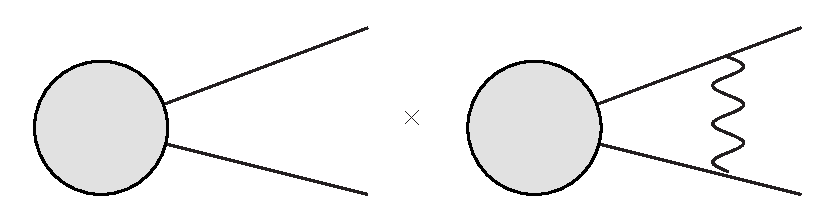
\includegraphics[width=0.17\linewidth]{./path-feynman/2.eps}
   \caption{Feynman diagrams}
\end{figure}

General case: common (position space) Feynman rules for interacting Green's functions $G_n (x_1, \dots, x_n)$

\section[Photon Propagator in Path Integrals]{Photon Propagator in Path Integrals\footnote{see also Ryder, Chap 7.1-2; P \& S, Chap 9.4}}
How can we derive the Feynman rule for photon propagator?
\begin{align}
   \frac{-ig^{\mu\nu}}{k^2 + i \epsilon}
\end{align}

What is the problem? The functional integral $\int \D A_\mu \euler^{iS[A]}$ incorporated the action
\begin{align}
   S &= \int \dd[4]{x} \left( - \frac{1}{4} F_{\mu\nu} F^{\mu\nu} \right) \notag\\ 
     &= \frac{1}{2} \int \dd[4]{x} A_\mu(x) \left( \partial^2 g^{\mu\nu} - \partial^{\mu} \partial^\nu \right) A_\nu(x) \notag\\
     &= \frac{1}{2} \int \frac{\dd[4]{k}}{(2\pi)^4} \tilde{A}_\mu (k) (-k^2 g^{\mu\nu} + k^\mu k^\nu) \tilde{A}_\nu (-k) 
\end{align}
This expression has a great deal of (interconnected) problems
\begin{enumerate}
   \item Assume the photon propagator $D_{\mu\nu} (x-y)$ to be solution of
         \begin{align*}
            \left( \partial^2 g^{\mu\nu} - \partial^\mu \partial^\nu \right)D_{\nu\lambda} (x-y) = i g^\mu_\lambda \delta^{(4)}(x-y) \\
            \shortintertext{multiply with partial derivative}
            \left( \partial^\nu \partial^2 - \partial^2 \partial^\nu \right) D_{\nu\lambda} = 0 \cdot \partial^\nu D_{\nu\lambda} \neq i \partial^\nu \delta^{(4)} (x-y)
         \end{align*}
         $D_{\nu\lambda}$ has no inverse (formally singular). The same holds in momentum space.
      \item We need this inverse for the derivation of the generating function with external currents.
      \item $\frac{1}{2} \int \frac{\dd[4]{k}}{(2\pi)^4} \tilde{A}_\mu (k) (-k^2 g^{\mu\nu} + k^\mu k^\nu) \tilde{A}_\nu (-k)$ vanished for all $\tilde{A}_\nu(k) = k_\mu \alpha(k)$
         all these field configurations have the same weight $1$ in $\int \D A_\mu \euler^{iS[A]}$. It will terribly diverge. 
      \item These configurations correspond to gauge transformation $\lag$ (also $S$) invariant under $A_\mu(x) \mapsto A_\mu(x) + \frac{1}{\euler} \partial_\mu \alpha(x) $. 
         Thus redundant (path-integral) integration over gauge equivalent configurations.
\end{enumerate}

Schematically to split each $A_\mu$ into some fixed $\bar{A}_\mu$ and a gauge transformation $\alpha$
\begin{align*}
   A_\mu (x) \mapsto \bar{A}_\mu (x), \alpha(x)
\end{align*}
then the path integral is given by
\begin{align*}
   Z = \int \D A_\mu \euler^{iS} \sim \int \D \bar{A}_\mu e^{iS} \int \D \alpha
\end{align*}
since $S$ is gauge invariant, i.e.~independent of $\alpha$.

The divergence stems from $\int\D \alpha$ which cancels in the ratio $W[j] = \frac{Z[j]}{Z[0]}$

The aim is to factorize of the gauge part in the path integral via a "smart integration" of the gauge-fixing as a constraint. This is called \underline{Faddeev-Popov method}.

\subsection[Factorization of Constraints]{Factorization of Constraints\footnote{Ryder, Chap 7.2}}
Externally simple example
\begin{align*}
   I &= \int \dd{x} \dd{y} \euler^{-(x^2 + y^2)}   \\
      \shortintertext{it is rotation invariant, use polar coordinates}
     &= \int \dd{\theta}\dd{r} r e^{-r^2}
   \shortintertext{$\int \dd{\theta} = 2\pi$ corresponds to $\int \D \alpha$ in the path integral.}
\end{align*}

A more general expansion for this separation
\begin{align*}
   I = \int \dd{\theta'} \int \dd{r} \int \dd{\theta} r \euler^{-r^2} \delta(\theta)
   \shortintertext{The delta function reduced the integration path to one along the x-axis ($\theta = 0$).}
\end{align*}

A more general path 
\begin{align}
f(\theta) = y\cos\theta - x \sin\theta = 0
\end{align}
i.e.~$\theta \neq 0$.

How can we include this constraint in path integral?
\begin{align}
   \delta (f(\theta)) &= \sum_i \left| \frac{\partial f(\theta_i)}{\partial \theta} \right|^{-1} \delta(\theta - \theta_i)
   \shortintertext{with $\theta_i$ the roots of $f(\theta).$}
   \theta_1 = \arctan(\frac{y}{x}) &\quad \theta_2 = \pi + \arctan(\frac{y}{x})  \notag\\
   \left| \frac{\partial f}{\partial \theta} \right| &= y \sin\theta + x \cos\theta = r = \left| \frac{\partial f}{\partial \theta} \right|_{\theta_1, \theta_2} \notag\\
   \shortintertext{thus} \notag
   \delta(f(\theta)) &= \frac{1}{r} \left( \delta(\theta-\theta_1) + \delta(\theta - \theta_2) \right) \notag\\
   \int \delta(f(\theta)) \dd \theta &= \frac{2}{r} = \frac{2}{\sqrt{x^2 + y^2}} \notag
   \shortintertext{rewrite this as $\Delta(r) \int \delta(f(\theta))\dd{\theta}  = 1$, i.e.~}
   \Delta (r) &= \frac{r}{2} = \frac{\sqrt{x^2 + y^2}}{2}
\end{align}

Note that $f(\theta)$ can simply be obtained by a rotation from $y$-axis
\begin{align*}
   y' &= y\cos\theta - x \sin\theta \\
   x' &= x\cos\theta + y \sin \theta \\
   x^2 + y^2 &= x'^2 + y'^2
\end{align*}

\begin{align*}
   \Delta(r) \int \dd{\theta} \delta(f(\theta)) &=1  \\
   \Delta \left(\sqrt{x'^2 + y'^2} \right) \int \dd{\theta} \delta(y')&= 1
\end{align*}
remember $y' = f(\theta) = y\cos\theta - x\sin\theta$.

Insert this unity into $I = \int \dd{x} \dd{y} \euler^{-(x^2 + y^2)}$
\begin{align*}
   I = \int \dd{\theta} \int \dd{x'} \dd{y'} \euler^{-(x'^2 + y'^2)} \Delta \left(\sqrt{x'^2 + y'^2} \right) \delta(y')
\end{align*}
It exhibits separation of variables made possible by the rotation invariance of the integral. The integral $\int \dd{x'} \dd{y'} \dots$ is independent of $\theta$, so $\int \dd{\theta}$ is simply an overall multiplication factor in integral.

Finally $\Delta(r)$ can also be rewritten as 
\begin{align}
   \Delta(r)^{-1} &= \int \dd{\theta} \delta(f(\theta)) \label{math:DeltaInv} \\
                  &= \int \delta(f(\theta)) \det \left|\frac{\dd{\theta}}{\dd f} \right| \dd{f} \notag\\
                  &= \det \left|\frac{\dd{\theta}}{\dd{f}} \right|_{f=0}\notag
                  \shortintertext{then we have the functional determinant}
   \Delta(r) &= \det \left| \frac{\dd{f}}{\dd{\theta}} \right|_{f=0}
\end{align}

\subsection{Gauge Fixing in a Path Integral}
Consider a gauge transformation 
\begin{align}
   A_\mu(x) \mapsto A_\mu^\alpha(x) = A_\mu(x) + \frac{1}{e} \partial_\mu \alpha(x)
\end{align}
and a gauge-fixing condition 
\begin{align}
   F[A_\mu] = 0
\end{align}

In analogy to the condition \ref{math:DeltaInv}
\begin{align}
   \Delta_F^{-1}[A_\mu] = \int \D \alpha \delta \left(F[A_\mu^\alpha] \right)
\end{align}
where $\delta$ is a $\delta$-functional.

$\Delta_F^{-1}[A_\mu]$ is gauge invariant
\begin{align*}
   \Delta_F^{-1} \left[ A_\mu^{\alpha'} \right] &= \int \D \alpha \delta \left( F [A_\mu^{\alpha+\alpha'}] \right) \\
   \shortintertext{group invariant measure $\alpha'' = \alpha + \alpha'$}
                        &= \int \D \alpha''  \delta \left( F[A_\mu^{\alpha''}] \right) = \Delta_F^{-1}[A_\mu]
\end{align*}

Insert $1 = \Delta_F [A_\mu] \int \D \alpha \delta(F[A_\mu^\alpha])$ into the path integral $Z$
\begin{align}
   Z &= \int \D A_\mu \euler^{iS[A_\mu]} \notag\\
     &= \int \D A_\mu \Delta_F[A_\mu] \int \D \alpha \delta \left( F[A_\mu^\alpha] \right) \euler^{iS[A_\mu]} \notag\\
   \shortintertext{using the gauge transformation $A_\mu \mapsto A_\mu^\alpha$}
     &= \int \D A_\mu^\alpha \Delta [A_\mu^\alpha] \int \D \alpha \delta \left( F[A_\mu^\alpha] \right)\euler^{iS[A^\alpha_\mu]} \notag \\
     \shortintertext{rename $A^\alpha_\mu = A_\mu$}
     &= \int \D \alpha \int \D A_\mu  \Delta_F [A_\mu] \delta \left( F[A_\mu] \right) \euler^{iS[A_\mu]} \label{math:zAlpha}
\end{align}

$S$ and $\Delta_F(\dots)$ are gauge invariant and $\D A_\mu^\alpha = \D A_\mu$, since
\begin{align*}
   Z &= \int \D A_\mu \euler^{iS[A_\mu]} \\
     &= \int \D A_\mu^{\tilde{\alpha}} \euler^{iS[A_\mu^{\tilde{\alpha}}]} \\
     &= \int \D A_\mu^{\tilde{\alpha}} \euler^{iS[A_\mu]}
\end{align*}
or $A_\mu \mapsto A_\mu^{\tilde{\alpha}}$ is just a shift of integration. Integrand of equation \ref{math:zAlpha} independent of gauge $\alpha$. Thus $\int \D \alpha$ can be moved in front and is therefore already separated!

Now use 
\begin{align}
   \Delta_F[A_\mu] = \det \left| \frac{\delta F}{\delta \alpha} \right|_{F=0}
\end{align}
We will apply gauge-fixing conditions of the form (generalization of Lorenz gauge)
\begin{align}
   F[A_\mu] &= \partial^\mu A_\mu + C(x) = 0
   \shortintertext{with $c(x)$ any scalar function. Thus }
   F[A_\mu^\alpha] &= F[A_\mu] + \frac{1}{e} \partial^2 \alpha(x) \\
   \Delta_F[A_\mu] &= \det \left| \frac{1}{e} \partial^2 \right| 
\end{align}
independent of $A_\mu$.
$\Delta_F[A_\mu]$ can be moved in front of the path integral. (Not valid in the non-abelian case.)

Since $Z$ and in the end, the physics does not depend on value of $C(x)$, we are free to have a linear combination of different $C(x)$. Now multiply equation (\ref{math:zAlpha}) with a weight$\int \D C \exp(\frac{-i}{2\xi}C^2 \dd{x})$.
After integrating $\int \D C$) and using $\delta \left( F[A_\mu] \right) = \delta \left( \partial^\mu A_\mu - C(x) \right)$
\begin{align}
   Z &= N \int \D A_\mu \exp{i \int \dd[4]{x} \left( \lag - \frac{1}{2\xi} \left( \partial_\mu A^\mu\right)^2  \right)} \\
   \lag_{\text{eff}} &= \lag + \lag_{\text{GF}} = - \frac{1}{4} F_{\mu\nu} F^{\mu\nu} - \frac{1}{2\xi} (\partial_\mu A^\mu)^2
\end{align}
with the gauge-fixing term in Lagrangian.

Now consider an n-point Green's function a la
\begin{align*}
   \braket{0 | T \left( O[A_\mu] \right)| 0}
\end{align*}

Coming back to our starting problem, to find photon propagator
\begin{align}
   \left( -k^2 g_{\mu\nu} + \left( 1- \frac{1}{\xi} \right) k_\mu k_\nu \right) \tilde{D}_F^{\nu\lambda}(k) = i\delta^\lambda_\mu \notag \\
   \shortintertext{possess the solution}
   \tilde{D}_{F}^{\mu\nu} (k) = \frac{-i}{k^2 + i\epsilon} \left( g^\mu\nu - (1-\xi) \frac{k^\mu k^\nu}{k^2} \right)
\end{align}
Most commonly used gauges Feynman gauge $\xi = 1$ and Landau gauge $\xi = 0$

\section[Path Integral Quantization of Fermion Fields]{Path Integral Quantization of Fermion Fields\footnote{see also Ryder Chap 6,7, P\& S, Chap 9.5}}
The fermionic fields anti-commute, therefore the integration over (complexed-valued) fermion fields is non-trivial.

\subsection[Grassmann Algebra]{Grassmann Algebra\footnote{see also F.A.Berezin, the method of second quantization, 1966}}
Consider an algebra $\mathcal{G}_n$ generated by n anticommuting generators $\theta_1, \dots, \theta_n$.
\begin{align}
   \theta_i \theta_j + \theta_j \theta_i = \left\{ \theta_i, \theta_j \right\} = 0
\end{align}
They are variables, not field operators (yet)!

Implicitly $\theta_i^2 = 0$ for all $i$ Thus a basis is given monomials (polynomial of first order of one term) $1; \theta_1, \dots, \theta_n; \theta_1 \theta_2, \dots \theta_{n-1}\theta_n; \dots; \theta_1\dots\theta_n$

Each element $F(\theta) \in \mathcal{G}_n$ can be expressed as a linear combination of these monomials.
\begin{align}
   F(\theta) = F^{(0)} + \sum_i F_i^{(1)} \theta_i + \dots + \sum_{i \dots k} F^{(n)}_{i,\dots,k} \theta_i \dots \theta_j \dots \theta_k
\end{align}
All coefficient are totally antisymmetric under exchange of the indices. We call elements with even (odd) monomials even (odd) algebra. Every $F(\theta)$ can be uniquely decomposed into a sum of even and odd monomials. Even elements \underline{commute} with each other and odd elements \underline{anti-commute} with each other.

In $\mathcal{G}_n$ we can define sums $F(\theta) + G(\theta) $ products $F(\theta) \cdot G(\theta) $ and functions $\euler^{F(\theta)} = 1 + F(\theta) + \frac{1}{2!} \left( F(\theta) \right)^2 + \dots$. All these therms can easily be expressed as linear combinations of moments.

\paragraph{Differentiation}
\begin{align}
   \pdv{\theta_j} \theta_i &= \delta_{ij} \\
   \pdv{\theta_i} c &= 0, \quad  c \in \Co \\
   \shortintertext{from anti-commutation relation and sign convention and derivative always acts on variable directly following}
   \pdv{\theta_i} (\theta_1 \dots \theta_n) &= \delta_{i1} \theta_2 \dots \theta_n - \delta_{i2} \theta_1 \theta_3 \dots \theta_n + \dots + (-1)^{n-1} \theta_1 \dots \theta_{n-1}
   \shortintertext{it has the consequence}
   \acomm{\pdv{\theta_i}}{\pdv{\theta_j}} &= 0 \\
   \acomm{\pdv{\theta_i}}{\theta_j} &= \delta{ij}
\end{align}
We can then read $\theta_i$ and $\pdv{\theta_j}$ as a representation of fermion creation and annihilation operators.

\paragraph{Integration}
The goal is to find generalization of functional integrals, so we only need the analogue of $\int_{-\infty}^{\infty} \dd{x}$, no need of finite integrals. First consider one single Grassmann variable $\theta$
\begin{align}
   \int \dd{\theta} f(\theta) &= \int \dd{\theta} \left( A + B \theta \right) \notag 
   \shortintertext{it should be a linear function of $A$ and $B$ because of linearity of integration. To enable variable shift $\theta \mapsto \theta + \eta$}
   \int \dd{\theta} \left( A + B\theta \right) &= \int \dd{\theta} \left( \left( A+b\eta \right) + B \theta \right) \notag \\
   \Rightarrow \int 1 \cdot \dd{\theta} &= 0 \\
   \shortintertext{in addition we define}
   \int \dd{\theta} \theta &= 1
   \shortintertext{in general}
   \int \dd{\theta_i} &= 0 \\
   \int \dd{\theta_i} \theta_j &= \delta_{ij} \\
   \acomm{\dd{\theta_i}}{\dd{\theta_j}} &= 0 = \acomm{\theta_i}{\dd{\theta_j}}
   \shortintertext{multiple integrals}
   \int \dd{\theta_n} \dots \dd{\theta_1} F(\theta) &= \int \dd{\theta_n} \dots \dd{\theta_1} \left( \sum^n_{i,\dots,k} F^{({n})}_{i\dots k} \theta_i \dots \theta_k \right) = n! F^{(n)}_{12\dots n}
\end{align}
All terms with $k<n$ vanish due to $\int \dd{\theta_i} = 0^n$
Note that differentiation and integration with respect to Grassmann variables yield same result.

\paragraph{Gaussian integrals} for \underline{even} numbers of generators and $A$ skew-symmetric matrix.
\begin{align}
   \int \dd{\theta_1} \dots \dd{\theta_n} \euler^{-\frac{1}{2} \theta_i A_{ij} \theta_j} = \sqrt{\det{A}} \label{math:grassmannGaussian}
\end{align}

Here consider only example for $n=2$, i.e.~$A_{11}=A_{22}=0$ and $A_{12}=-A_{21}$
\begin{align*}
   \euler^{-\frac{1}{2}\theta_i A_{ij} \theta_j} &= \euler^{-\frac{1}{2} \left( \theta_1 \theta_2 A_{12} + \theta_2 \theta_1 A_{21} \right)} \\
                                                 &= \euler^{-A_{12}\theta_1\theta_2} \\
                                                 &= 1 - A_{12} \theta_1 \theta_2
                                                 \shortintertext{hence}
   \int \dd{\theta_1} \dd{\theta_2} \euler^{-\frac{1}{2}\theta_i A_{ij} \theta_j} &= \int \dd{\theta_1} \dd{\theta_2} \left(1 - A_{12} \theta_1 \theta_2\right) = A_{12} \\
                                                                                  &= \sqrt{\det{A}}
\end{align*}

There is a subtlety in the equation (\ref{math:grassmannGaussian}). Unlike two dimensional case where we only consider the terms up to linear term, we need to take care of higher order terms in higher dimension, otherwise the integral vanishes!
There is a subtlety in the equation. Unlike two dimensional case where we only consider the terms up to linear term, we need to take care of higher order terms in higher dimension, otherwise the integral vanishes!

For each skew-symmetric matrix of even rank, the determinant is a perfect square while for each skew-symmetric matrix of odd rank, $\det{A} = 0$. $\sqrt{\det{A}}=$ Pfaffian form
\begin{align*}
   n&=2 \quad &&P = A_{12} = \frac{1}{2}\epsilon A_{ij} \\
   n&=4 \quad &&P = A_{12}A_{34} - A_{13}A_{24} + A_{14}A_{23} = \frac{1}{8}\epsilon_{ijkl} A_{ij}A_{kl}
\end{align*}

\subsection{Fermion Fields}
Definition of Grassmann fields as functions of space-time, whose values are anti-commuting numbers, .e.g.
\begin{align}
   \psi (x) = \sum_i \psi_i \phi_i (x) 
\end{align} 
with $\psi_i \in \mathcal{G}, \phi_i \in \Co$. For Dirac fields, $\phi_i$ are 4-component spinors.

As in the scalar case, to add external sources $\eta, \bar{\eta}$ to the Dirac Lagrangian
\begin{align}
   \lag = \bar{\psi} \left( i\slashed{\partial} - m \right)\psi + \bar\psi \eta + \bar{\eta} \psi
\end{align}
Obviously the sources must be Grassmann valued $\acomm{\eta}{\eta} = \acomm{\eta}{\bar{\eta}} = \acomm{\bar{\eta}}{\bar{\eta}} = \acomm{\psi}{\eta} = \acomm{\bar\psi}{\eta} = \acomm{\psi}{\bar\eta} = \acomm{\bar\psi}{\bar\eta} = 0$. 

Vacuum to vacuum transition amplitude in presence of external sources
\begin{align}
   \braket{0|0}^{\eta\bar{\eta}} = \int \D \bar{\psi} \D \psi \exp{i\int \dd[4]{x} \left[ \bar{\psi} (i\slashed{\partial} - m)\psi + \bar{\eta}\eta + \bar{\psi} \eta \right]}
\end{align}

Determine classical solution from the least-action principle
\begin{align}
   \psi_{\cl} (x) = i \int \dd[4]{y} S_F(x-y) \eta(y) \\
   \bar\psi_{\cl} (x) = i \int \dd[4]{y} \bar\eta(y)S_F(x-y)  
\end{align}
with already known Dirac propagator
\begin{align}
   S_F(x-y) = \int \frac{\dd[4]{k}}{(2\pi)^4} \frac{i(\slashed{k}+m)}{k^2 - m^2 +i\epsilon} \euler^{-ik(x-y)}
\end{align}
as the Green's function of the Dirac operator $(i\slashed{\partial} - m)$.

By expansion of $\psi(x)$ around the classical solution $\psi_\cl(x)$ we find, like in the scalar case,
\begin{align}
   \braket{0|0}^{\eta, \bar{\eta}} &= \euler^{iS_\cl} \braket{0|0}^{\eta=\bar{\eta}=0} 
   \shortintertext{and classical action can be rewritten as}
   iS_\cl &= i\int \dd[4]{x} \left[ \bar{\psi}_\cl \left( i \slashed{\partial} - m \right) \psi_\cl + \bar{\psi}_\cl \eta + \bar\eta \psi_\cl \right] \\
          &= - \int \dd[4]{x} \dd[4]{y} \bar{\eta}(x) S_F(x-y) \eta(y)
          \shortintertext{hence the generating functional for the free Dirac field is given as}
   W_0 [\eta, \bar\eta] &= \frac{\braket{0|0}^{\eta, \bar\eta}}{\braket{0|0}^{\eta=\bar\eta=0}} = \exp{-i\int\dd[4]{x}\dd[4]{y}\bar\eta(x)S_F(x-y)\eta(y)}
\end{align}
 
Derive n-point functions from generating functional
\begin{align}
   \braket{0 | T \psi(x) \bar \psi(y) | 0} = \frac{1}{i} \frac{\delta}{\delta \eta(y)} \frac{1}{i} \frac{\delta}{\delta \bar\eta(x)} \eval{W_0[\eta, \bar\eta]}_{\eta=\bar\eta=0}
\end{align}

\subsection{QED}
Lagrangian given as 
\begin{align}
   \begin{split}
   \lag_{\text{QED}} &= \bar\psi \left( i \slashed{\text{D}} -m \right)\psi - \frac{1}{4}F^{\mu\nu} F_{\mu\nu} - \frac{1}{2\xi} \left( \partial_\mu A^\mu \right)^2 \\
                     & = \bar\psi \left( i \slashed{\partial} -m \right)\psi - \frac{1}{4}F^{\mu\nu} F_{\mu\nu} - \frac{1}{2\xi} \left( \partial_\mu A^\mu \right)^2 - e \bar\psi \gamma^\mu \psi A_\mu \\
                     &= \lag_0 + \lag_{\text{GF}} - e \bar\psi \gamma^\mu \psi A_\mu 
   \end{split}
\end{align}
Expand the exponential of the interaction term.
\begin{align*}
   \exp{i\int\dd[4]{x} \lag_{\text{QED}}} = \exp{i\int \dd[4]{x} \left( \lag_0 + \lag_{\text{GF}} \right)} \cdot \left[ 1-ie\int \dd[4]{x} \bar\psi \gamma^\mu \psi A_\mu +\dots \right]
\end{align*}

Feynman rules (position space)
\begin{align}
   \feynmandiagram[horizontal=a to b]{
      a --[fermion, momentum=\(p\)] b;
   }; 
   &= \int \frac{\dd[4]{p}}{(2\pi)^4} \frac{i (\slashed{p}+m)}{p^2 - m^2 + i\epsilon} \euler^{-ip(x-y)} \\
   \feynmandiagram[horizontal=a to b]{
      a --[photon, momentum=\(p\)] b;
   }; 
   &= \int \frac{\dd[4]{p}}{(2\pi)^4} \frac{-i}{q^2 + i\epsilon} \left( g^{\mu\nu} - (1-\xi)\frac{q^\mu q^\nu}{q^2} \right) \euler^{-ip(x-y)} \\
   \feynmandiagram[small, horizontal=a to b, inline=(a.base)]{
      a [particle={\(\mu\)}] --[photon] b -- [fermion] c,
      b --[anti fermion] d,
   };
   &= -ie\gamma^\mu \int \dd[4]{x}
\end{align}

Generating functional for QED
\begin{align}
   Z[j_\mu, \eta, \bar\eta] &=  \int \D A_\mu \D \bar{\psi} \D \psi \exp{i\int \dd[4]{x} \left( \lag_0 + \lag_{\text{GF}} + \lag_{\text{int}} + j_\mu A^\mu + \bar\psi \eta + \bar\eta \psi \right)} \\
   Z[j_\mu, \eta, \bar\eta] &= \frac{Z[j_\mu, \eta,\bar\eta]}{Z[j_\mu=0, \eta=\bar\eta=0]}
\end{align}

\section{Generating Functional for Fully Connected Green's Functions}
Return to scalar theory for simplicity. In section 2.2 we calculated $4$-point function to $\lambda^0$
\begin{align}
   \braket{0 | T \phi(x_1)\phi(x_2)\phi(x_3)\phi(x_4) | 0} &=  D_F (x_3 - x_4) D_F(x_1 - x_2) + D_F(x_2 - x_4) D_F(x_1-x_3) \\
   &\quad + D_F(x_1 - x_4) D_F(x_2-x_3)
\end{align}

To next order in perturbation theory $\mathcal{O}(\lambda^1)$
\begin{align}
   \braket{0 | T \phi(x_1)\phi(x_2)\phi(x_3)\phi(x_4) | 0} &=
   3 \vcenter{\hbox{
      \feynmandiagram[small, horizontal=a to b, layered layout, inline=(e.base)]{
         a[dot] -- b -- c[dot],
         d[dot] -- e -- f[dot],
      {[same layer] b --[opacity=0] e,},
};}}
- 3i \lambda \vcenter{\hbox{
      \feynmandiagram[small, horizontal=a to b, layered layout, inline=(e.base)]{
         a[dot] -- b -- c[dot],
         d[dot] -- e -- f[dot],
      {[same layer] b --[opacity=0] e,},
      {[same layer]e --[half left] x[nudge=(90:6mm)] --[half left] e,}
};}}
- i \lambda  \vcenter{\hbox{
   \feynmandiagram[small, horizontal=a to b]{
      {a[dot], c[dot]}-- x[dot] -- {b[dot], d[dot]};
   };}}
   + \order{\lambda^2}
\end{align}
only the last term is fully connected and contributes to T-matrix!

There exists a generating functional $E[j]$ that only generates the fully connected diagrams
\begin{align}
   i E[j] = \ln(Z[j])
\end{align}
\textbf{Note} that often in the literature, $E[j]$ is often called $W[j]$!

To show that $E[j]$ in $\lambda\phi^4$ generates no disconnected contributions in the $2$- and $4$-point functions!
\paragraph{$2$-point function}
\begin{align*}
   \frac{\delta^2 iE[j]}{i\delta j(x_1) i \delta j(x_2) } &=  \frac{1}{Z} \frac{\delta^2 Z}{i\delta j(x_1) i \delta j(x_2)} - \frac{1}{Z^2} \frac{\delta Z}{i \delta j(x_1)} \frac{\delta Z}{i \delta j(x_2)}
   \shortintertext{since $Z$ is quadratic in $j$, for $j=0$ term with one derivative drops put. Hence}
   \eval{\frac{\delta^2 iE[j]}{i\delta j(x_1) i \delta j(x_2) }}_{j=0}  &= \eval{\frac{1}{Z} \frac{\delta^2 Z}{i\delta j(x_1) i \delta j(x_2)}}_{j=0}\\
                                                         &= D_F(x-y)
\end{align*}
there is (to arbitrary order in $\lambda$) the propagator. It doesn't have disconnected poles.

\paragraph{$4$-point function}
\begin{align*}
   & \eval{\frac{\delta^4 iE[j]}{i\delta j(x_1) i \delta(x_2) i\delta j(x_3) i \delta(x_4)}}_{j=0}  \\
   &= \frac{1}{Z} \eval{\frac{\delta^4 Z[j]}{\delta j(x_1) \delta(x_2) \delta j(x_3) \delta(x_4)}}_{j=0}  - \eval{\frac{1}{Z^2} \frac{\delta^2 Z}{ \delta j(x_1) j(x_2)} \frac{\delta^2 Z}{\delta j(x_3) \delta j(x_4)}}_{j=0}- \eval{\frac{1}{Z^2} \frac{\delta^2 Z}{ \delta j(x_1) j(x_3)} \frac{\delta^2 Z}{\delta j(x_2) \delta j(x_4)}}_{j=0} \\ & \quad - \eval{\frac{1}{Z^2} \frac{\delta^2 Z}{ \delta j(x_1) j(x_4)} \frac{\delta^2 Z}{\delta j(x_2) \delta j(x_3)}}_{j=0}
\\
             & = \braket{0 | T \phi_1 \phi_2 \phi_3 \phi_4 | 0} - \braket{0|T\phi_1 \phi_2|0} \braket{0|T\phi_3 \phi_4|0} - \braket{0|T\phi_1 \phi_3|0}\braket{0|T\phi_2 \phi_4|0} - \braket{0|T\phi_1 \phi_4|0} \braket{0|T\phi_2 \phi_3|0}  \\
             &=
             \left(\vcenter{\hbox{
      \feynmandiagram[small, horizontal=a to b, layered layout, inline=(e.base)]{
         a[dot] -- b -- c[dot],
         d[dot] -- e -- f[dot],
      {[same layer] b --[opacity=0] e,},
      };}}
      + 2 \text{ crossed}
      \right)
      - \frac{i\lambda}{2} \left( \vcenter{\hbox{
      \feynmandiagram[small, horizontal=a to b, layered layout, inline=(e.base)]{
         a[dot] -- b -- c[dot],
         d[dot] -- e -- f[dot],
      {[same layer] b --[opacity=0] e,},
      {[same layer]e --[half left] x[nudge=(90:6mm)] --[half left] e,}
   };}} + 5 \text{ crossed} \right)
   - \frac{i \lambda }{4!} \left( \vcenter{\hbox{
   \feynmandiagram[small, horizontal=a to b]{
      {a[dot], c[dot]}-- x[dot] -- {b[dot], d[dot]};
   };}} + 23 \text{ crossed} \right) \\
             & \quad - \left( 
                \feynmandiagram[small, horizontal=a to b]{a[dot,label=\(1\)] -- b[dot, label=\(2\)]}; 
             - \frac{i\lambda}{2} 
             \feynmandiagram[small, horizontal=a to b, layered layout, inline=(a.base)]{a[dot, label=\(3\)] -- b[dot] -- c[dot,label=\(4\)]; {[same layer]b--[half left]x[nudge=(90:6mm)]--[half left]b} };
            \right)
            \cdot \left( 
                \feynmandiagram[small, horizontal=a to b]{a[dot,label=\(3\)] -- b[dot, label=\(4\)]}; 
             - \frac{i\lambda}{2} 
             \feynmandiagram[small, horizontal=a to b, layered layout, inline=(a.base)]{a[dot, label=\(1\)] -- b[dot] -- c[dot,label=\(2\)]; {[same layer]b--[half left]x[nudge=(90:6mm)]--[half left]b} };
            \right)
            - 2 \text{ crossed}
\end{align*} 
Indeed only the fully connected term survive!

So define in general the "connected" or "irreducible" $n$-point function by
\begin{align}
   \braket{0 | T\phi(x_1) \dots \phi(x_n) | 0 }_\text{c} = \frac{1}{i} \frac{\delta}{\delta j(x_1)} \dots \frac{1}{i} \frac{\delta}{\delta j(x_n)} i E[j]
\end{align}
We have shown that
\begin{align*}
   \braket{0 | T \phi_1 \phi_2 \phi_3 \phi_4 | 0} = \braket{0 | T \phi_1 \phi_2 \phi_3 \phi_4 | 0}_c + \sum_{P} \braket{0 | T\phi_{i_1}\phi_{i_2}}_\text{c} \braket{0 | T \phi_{i_3} \phi_{i_4} | 0}_\text{c}
\end{align*}

Example for $6$-point function
%TODO

\section{Effective action and Legendre Transform}
$iE[j]$ is generating functional for irreducible Green's functions. Formally 
\begin{align}
   iE[j] = \sum_n \frac{i^n}{n!} \dd[4]{x_1} \dots \dd[4]{x_n} G_\text{c}(x_1,\dots,x_n) j(x_1) \dots j(x_n)
\end{align} 
Remember the LSZ reduction formula. It is the relation between S-matrix and Green's function
\begin{align}
   {}_{\text{out}} \braket{k_1 \dots k_m | k_{m+1} \dots k_n}_{\text{in}} = \text{disconnected terms} + \prod_{j=1}^n \left( \frac{iZ}{k^2_j - m^2 +i \epsilon} \right)^{-1} \sqrt{Z}^n G(k_1, \dots, k_n)
\end{align} 
Conclusion is that n-point Green's function contain \text{poles} in all external legs. S-matrix elements are \text{amputated} Green's functions.
In the following to derive generating functional for \underline{amputated}, \underline{fully connected} (\underline{one-particle-irreducible}) Green's functions. It leads to "effective action".

\paragraph{Define} the \underline{classical field}
\begin{align}
   \phi(x) = \frac{\delta}{\delta j(x)} E[j]
\end{align}
For $j \neq 0$, $\phi=\phi[j]$ can in principle be inverted to $j=j[\phi]$.

\underline{Effective action} is Legendre transform of $E[j]$
\begin{align}
   \Gamma[\phi] = E - \eval{\int \dd[4]{x} j(x) \phi(x)}_{j=j[\phi]}
\end{align}

$j(x)$ can be recovered from $\Gamma$ by functional derivation with respect to $\phi$
\begin{align}
   \frac{\delta}{\delta \phi(x)} \Gamma[\phi] = -j(x)
\end{align}
Note that $E=E[j[\phi]]$, so this calculation is not quite as trivial as it seems.

\paragraph{Define} $\Gamma(x_1, \dots, x_n)$ through the formal expansion
\begin{align}
   \Gamma[\phi] = - \sum \frac{(-i)^n}{n!} \int \dd{x_1} \dots \dd{x_n} \Gamma(x_1, \dots, x_n) \phi(x_1) \dots \phi(x_n)
\end{align}
$\Gamma(x_1,\dots, x_n)$ can be obtained from $\Gamma[\phi]$ by repeated function derivative with respect to $\phi(x_i)$.

Calculate first
\begin{align*}
   \frac{\delta}{\delta \phi(y)} \phi(y) &= \delta(x-y)  \\
                                         &= \frac{\delta}{\delta \phi(y)} \left( \frac{\delta}{\delta j(x)} E[j] \right)
                                         \shortintertext{use the chain rule}
                                         &= \int \dd[4]{z} \frac{\delta^2 E}{\delta j(x) \delta j(z)} \frac{\delta}{\delta \phi(y)} j(z)  \\
                                         &= -i \int \dd[4]{z} G_\text{c}(x-z) \Gamma(y-z)
\end{align*}
Fourier transform the result we have $i=\tilde{G}(p)\tilde{\Gamma}(p)$, or $\tilde{\Gamma}(p) = Z^{-1} (p^2 - m^2)$. Differentiate this once again
\begin{align*}
   \frac{\delta^2 \phi(x)}{\delta \phi(x) \delta(y)} &= 0 \\
                                                     &= \int \dd[4]{z} \dd[4][v] \left[ \frac{\delta^3 E}{\delta j(x) \delta j(z) \delta(v)} \frac{\delta j(z)}{\delta \phi(y)} \frac{\delta j(v)}{\delta \phi(n)}\right] + \int \dd[4]{z} \frac{\delta^2 E}{\delta j(x) \delta j(z)} \frac{\delta^2 j(z)}{\delta \phi(y) \delta\phi(x)} \\
                                                     &= -\int \dd[4]{z} \dd[4]{v} G(x,z,v) \Gamma(z,y) \Gamma(v,u) - \int \dd[4]{z} G(x,z) \Gamma(z,y,x) = 0
                                                     \shortintertext{multiply with $\int \dd[4]{x} \Gamma(x, \omega)$, use $\int \dd[4]{x} \Gamma(x-\omega) G(x-z) = i \delta(\omega -z)$}
   i \Gamma(\omega, y,u) &= \int \dd[4]{z}\dd[4]{v}\dd[4]{x}G(x,z,v) \Gamma(z,y) \Gamma(x,\omega) \Gamma(u,v)
   \shortintertext{graphically}
                         &\includegraphics[width=0.7\linewidth]{./3point-IR/1.eps}
\end{align*}
In word, $\Gamma(\omega,y,u)$ is the 1-particle irreducible version of $G(x,z,v)$!

%%%%%%%%%%%%%%%%%%%%%%%%%%%%%%%%%%%%%%%%%%%%%%%%%%%%%%%%%%%%%%%%%
% Lecture date: 19-11-06
%%%%%%%%%%%%%%%%%%%%%%%%%%%%%%%%%%%%%%%%%%%%%%%%%%%%%%%%%%%%%%%%%

\section{Ward-Takahashi Identity for QED}
Ward Takahashi identities are relations between one-particle irreducible vertex functions and propagators that hold to all orders in perturbation theory. It is in fact consequence of gauge invariance. It also plays key role in the proof of renormalizability of QED.

Generating functional of QED
\begin{align}
   Z[j_\mu, \eta, \bar{\eta}] &= N \int \D A_\mu \D \phi \D \bar\psi \exp{i\int \dd[4]{x} \lag_{\text{eff}}} \\
   \begin{split}
      \lag_{\text{eff}} &= \underbrace{-\frac{1}{4} F_{\mu\nu}F^{\mu\nu} + \bar{\psi} \left[ i \left( \slashed{\partial} + ie \slashed{A} \right)  - m\right]\psi}_{\lag} \\
                        &\quad  \underbrace{- \frac{1}{2\xi} (\partial_\mu A^\mu)^2 + j_\mu A^\mu + \bar\psi \eta + \bar\eta \psi}_{\lag_1}
   \end{split}
\end{align}
Two observations are seemly contradicting to each other
\begin{itemize}
   \item $\lag_{\text{eff}}$ is obviously \underline{not} gauge invariant, since we have introduced a gauge fixing term.
   \item On the other hand, physics as expressed through Green's functions \underline{must} be independent of gauge.
\end{itemize}
This non-trivial connection leads to differential equation for $Z$!

Consider infinitesimal gauge transformation
\begin{align*}
   A_\mu &\mapsto A_\mu + \partial_\mu \Lambda \\
   \psi &\mapsto \psi - ie \Lambda \psi \\
   \bar\psi &\mapsto \bar\psi + ie \Lambda \bar\psi
\end{align*}

In the decomposition $\lag + \lag_1$, all the changes are induced via $\lag_1$ ($\lag$ is gauge invariant)
\begin{align*}
   \delta \int \dd[4]{x} \lag_{\text{eff}} = \delta \int \dd[4]{x} \lag_1 = \int \dd[4]{x} \left[ -\frac{1}{\xi} (\partial_\mu A^\mu) \partial^2 \Lambda + j_\mu \partial^\mu \Lambda - ie \Lambda (\bar\eta \psi - \bar\psi \eta) \right]
\end{align*}
Hence the change in $Z[j, \eta, \bar\eta]$ is
\begin{align*}
   \delta Z[j, \eta,\bar\eta] &= N \int \D A_\mu \D \psi \D \bar\psi \exp{i\int \dd[4]{x} \lag_\text{eff}} \\
                              &\quad \times i \int \dd[4]{x} \left[ -\frac{1}{\xi} \partial^2 (\partial_\mu A^\mu) - \partial_\mu j^\mu - ie (\bar\eta \psi - \bar\psi \eta) \right]\Lambda(x)
\end{align*}

As $\Lambda(x)$ is arbitrary, the term is bracket needs to vanish. Take this bracket in front of the functional $Z$ using
\begin{align*}
   \psi &\mapsto \frac{1}{i} \fdv{\bar{\eta}}  \\
   \bar\psi &\mapsto -\frac{1}{i} \fdv{{\eta}}  \\
   A_\mu &\mapsto \frac{1}{i} \fdv{j^\mu}
\end{align*}

\begin{align}
   \left[ \frac{i}{\xi} \partial^2(\partial_\mu \fdv{j_\mu}) - \partial_\mu j^\mu - e \left( \bar\eta \fdv{\bar\eta} - \eta \fdv{\eta} \right) \right]Z[j, \eta, \bar\eta] &= 0 \notag
   \shortintertext{Transform this into PDE for generating functional of irreducible Green's functions $Z = \euler^{iE}$}
   - \frac{1}{\xi} \partial^2 \left(\partial_\mu \fdv{E}{j_\mu} \right) - \partial_\mu j^\mu - ie \left( \bar\eta \fdv{E}{\bar\eta}- \eta \fdv{E}{\eta} \right) &= 0 \label{math:wardPDE}
\end{align}

Finally use the effective action to derive relations for irreducible amputated vertex functions
\begin{align}
   \Gamma[A_\mu, \psi, \bar\psi] = E[j_\mu, \eta, \bar\eta] - \int \dd[4]{x} \left( j_\mu A^\mu + \bar\eta \psi + \bar\psi \eta \right)
\end{align}

\begin{align*}
   \fdv{\Gamma}{A_\mu} &= -j^\mu  \quad \fdv{E}{j^\mu} = A_\mu \\
   \fdv{\Gamma}{\psi} &= + \bar\eta \quad \fdv{E}{\bar\eta} = \psi \\
   \fdv{\Gamma}{\bar\psi} &= - \eta \quad \fdv{E}{\eta} = - \bar{\psi}
\end{align*}

After the replacement, equation \ref{math:wardPDE} becomes
\begin{align}
   \left[  \frac{1}{\xi} \partial^2 \partial_\mu A^\mu - \partial_\mu \fdv{\Gamma}{A_\mu} + ie \left( \bar \psi \fdv{\Gamma}{\bar\psi} + \fdv{\Gamma}{\psi}\psi \right)\right] &= 0
\end{align}
Take functional derivative $\fdv{\bar\psi} \fdv{\psi}$ and subsequently put $\bar\psi = \psi = A_\mu = 0$
\begin{align}
   - \partial_x^\mu \frac{\delta^3 \Gamma}{ \delta \bar\psi(x_1) \delta \psi(y_1) \delta A^\mu(x)} &= -ie \delta^{(4)}(x-x_1) \frac{\delta^2 \Gamma}{\delta \bar\psi(x_1) \delta \psi(y_1)} + ie \delta^{(4)} (x-y_1) \frac{\delta^2 \Gamma}{\delta\bar\psi(x_1) \delta \psi(y_1)} \label{math:threepointPDE}
\end{align}

This becomes more intuitive in momentum space. First define
\begin{align}
   \int \dd[4]{x} \dd[4]{x_1} \dd[4]{y_1} \exp[i(p'x_1 - py_1 - qx)] \frac{\delta^3 \Gamma}{ \delta \bar\psi (x_1) \delta \psi(y_1) \delta A^\mu(x)} = e (2\pi)^4(p'-p-q) \Gamma(p, q, p')
\end{align}
Know already the one-particle irreducible two-point function
\begin{align}
   \int \dd[4]{x_1} \dd[4]{y_1} \exp[i(p'x_1 - py_1)] \frac{\delta^2 \Gamma }{\delta \bar\psi (x_1) \delta \psi(y_1)} = - (2\pi)^4 \delta^{(4)} (p'-p) i S_F^{-1}(p) 
\end{align}
Multiply \ref{math:threepointPDE} with $\exp[i(p'x_1 - py_1 - qx)]$ and integrate over $x$, $x_1$ and $y_1$
\begin{align}
   q_\mu \Gamma^\mu(p,q,p+q) = i S_F^{-1}(p+q) - i S_F^{-1}(p)
\end{align}
This is \underline{Ward Takahashi identity}.

Graphically
\begin{align*}
   q^\mu
   \feynmandiagram[small, inline=(b.base), horizontal=b to c] {
      a[label=\(p+q\)] --[anti fermion] b [blob, label={270:\(\Gamma\)}] --[photon] c[label=270:\(q\)],
      b --[anti fermion] d[label=270:\(p\)],
}; =
   \feynmandiagram[layered layout, small, vertical = a to b, inline=(b.base)]{
   a --[anti fermion] b[blob] --[anti fermion]c[label=0:\(p+q\)],};
   -  \; \feynmandiagram[layered layout, small, vertical = a to b, inline=(b.base)]{
   a[label=0:\(p\)] --[anti fermion] b[blob] --[anti fermion]c,};
\end{align*}

At lowest order in QED
\begin{align*}
   S_F(p) &= \frac{i}{\slashed{p} - m} \\
   \Gamma^\mu (p,q,p+q) &= \gamma^\mu  \\
   \slashed{q} &= (\slashed{p} - \slashed{q} - m) - (\slashed{p} - m)
\end{align*}

In the limit $q^\mu \rightarrow 0$, we obtain \underline{Ward identity}
\begin{align}
   \Gamma^\mu (p,0,p) = \pdv{iS_F^{-1}}{p_\mu}
\end{align}

There are more Ward identities that can be derived using different functional derivatives. Start again with \ref{math:wardPDE} and differentiate with respect to $j_0(y)$, then put $\eta = \bar\eta = j = 0$
\begin{align}
   - \frac{1}{\xi} \partial^2 \partial_x^\mu \frac{\delta^2 E}{\delta j^\mu (x) \delta j^\nu (y)} &= \partial^\mu_x g_{\mu\nu} \delta^{(4)}(x-y) \notag
   \shortintertext{Remember photon propagtor is given by}
   \frac{i \delta^2 E}{i \delta j^\mu(x) i \delta j^\nu (y)} &= \braket{0 | T A_\mu(x) A_\nu(y) | 0} =  G_{\mu\nu}(x-y) \notag\\ 
   \frac{1}{\xi} \partial^2 \partial_x^\mu G_{\mu\nu}(x-y) &= i\partial_x^\mu g_{\mu\nu} \delta^{(4)}(x-y)
   \shortintertext{After Fourier transform}
   \frac{i}{\xi} k^2 k^\mu \tilde{G}_{\mu\nu}(k) &= k_\nu
\end{align}
Again it is true to all orders in perturbation theory. To say that the longitudinal component of $G_{\mu\nu}$ is fixed and not modified by interactions
\begin{align}
   \tilde{G}_{\mu\nu}(k) &= \left( g_{\mu\nu} - \frac{k_\mu k _\nu}{k^2} \right)G_T(k^2) + \frac{k_\mu k_\nu}{k^2} G_L(k^2)
\end{align}
with Ward identity
\begin{align}
   \frac{i}{\xi} k^2 G_L(k^2) k_\nu &= k_\nu \notag \\
   G_L(k^2) &= \frac{-i\xi}{k^2} \notag
\end{align}

Propagator at leading order
\begin{align*}
   \hat{G}_{\mu\nu}(k) &= \frac{-i}{k^2} \left( g_{\mu\nu} - (1-\xi) \frac{k_\mu k_\nu}{k^2} \right) \\
   G_T(k^2) &= \frac{-i}{k^2} \\
   G_L(k^2) &= - \frac{i\xi}{k^2}
\end{align*}

We will make heavy use of the fact Ward Takahashi identities hold to all orders in the following sections on the renormalization of QED.

\section{Renormalization of QED I: Divergences and Dimensional Analysis}
It is known from QFT course last term that loop diagrams are often (UV-)divergent. To obtain a sensible theory, need to \underline{regularise} these divergences and remove or absorb them by renormalization.

Analyse divergences structure of QED by \underline{dimensional analysis}. Superficial degree of divergences $D$ of a Feynman diagram with 
\begin{itemize}
   \item  $d$ space dimension
   \item  $L$ number of loops
   \item  $P_\gamma$ number of photon propagators
   \item  $P_e$ number of electron propagators
   \item  $N_\gamma$ number of external photons
   \item  $N_e$ number of external electrons
   \item  $V$ number of vertices
\end{itemize}

An arbitrary diagram contains the integral like
\begin{align}
   \int \frac{\dd[d]k_1 \dots \dd[d]{k_L}}{(\slashed{k}_{i_1} - m) \dots (\slashed{k}_{i_{P_e}}) k^2_{j_1} \dots k^2_{j_{P_\gamma}}} \sim k^D \notag
   \shortintertext{thus}
   D = dL - 2 P_\gamma - P_e
\end{align}

We want to eliminate $L$, $P_\gamma$ and $P_e$ in favour of $V$, $N_\gamma$ and $N_e$
\begin{itemize}
   \item $L$ is the number of undetermined momenta
      \begin{align}
      L = P - V + 1 = P_\gamma + P_e - V + 1
      \end{align}
   \item Each vertex is connected to $2$ electron and $1$ photon line. External lines are attached to $1$ vertex, internal to $2$ vertices. 
      \begin{align}
         V = 2P_\gamma + N_\gamma = \frac{1}{2}(2P_e + N_e)
      \end{align}
\end{itemize}

Put together
\begin{align}
   D &= d + V \left( \frac{d-4}{2} \right) - N_e \left( \frac{d-1}{2} \right) - N_\gamma \left( \frac{d-2}{2} \right)
   \shortintertext{for $d=4$}
   D &= 4 - \frac{3}{2} N_e - N_\gamma
\end{align}
In four dimension, $D$ is independent of number of vertices, only dependent on $N_e$ and $N_\gamma$. $D \geq 0$ only  for certain, finite "small" $N_e$ and $N_\gamma$.

There are three different categories 
\begin{itemize}
   \item $d < 4$ super-renormalizable $\Leftrightarrow [e] > 0$
   \item $d = 4$ renormalizable $\Leftrightarrow [e] = 0$
   \item $d > 4$ non-renormalizable$\Leftrightarrow [e] < 0$
\end{itemize}

Mass dimension of coupling constant $[\psi] = (d-1)/2$ and $[A_\mu] = (d-2)/2$. Interaction $e A_\mu \bar\psi \psi$ leads to $[e] = 2 - d/2$

Fermi theory of weak interaction contains the interaction term $G_F \left( \bar\psi \gamma_\mu (1-\gamma_5)\psi \right) \left( \bar\psi \gamma^\mu (1-\gamma_5) \psi \right)$. Coupling constant has negative mass dimension $[G_F] = -2$, non-renormalizable.
\begin{align*}
   \feynmandiagram[medium, baseline=(v1), horizontal=v1 to v2]{
      i1[particle=\(u\)] --[anti fermion] v1[dot, label=\(g\)] --[charged scalar, label=\(W^-\)] v2[dot, label=\(g\)] --[fermion] f1[particle=\(e^-\)],
      i2[particle=\(d\)] --[fermion] v1,
      v2 --[anti fermion] f2[particle=\(\nu_e\)],
   }; \sim
   \frac{g^2}{q^2 - M^2_W} \approx \frac{g^2}{M_W^2} = G_F
\end{align*}

Back to QED in $d=4$; divergent amplitudes
\begin{enumerate}[label=(\alph*)]
	\item \label{item:a} $\begin{aligned}[t]\feynmandiagram[small]{a[blob];}; \quad D &=4 \end{aligned}$
   \item \label{item:b} $\begin{aligned}[t]\feynmandiagram[small, horizontal=a to b, inline=(b.base)]{a[blob] --[photon] b;}; \quad D &=3\end{aligned}$
	\item \label{item:c}$\begin{aligned}[t]\feynmandiagram[small, horizontal=a to b, layered layout, inline=(b.base)]{a --[photon] b[blob] --[photon] c;}; \quad D &=2\end{aligned}$
	\item \label{item:d}$\begin{aligned}[t]\feynmandiagram[small, horizontal=a to c, spring layout, inline=(b.base)]{a --[photon] b[blob] --[photon] c; d --[photon] b;}; \quad D &=1\end{aligned}$
   \item \label{item:e}$\begin{aligned}[t]\feynmandiagram[small, horizontal=a to c, layered layout, inline=(b.base)]{a --[photon] b[blob] --[photon] c; d --[photon] b --[photon] e;}; \quad D &=0\end{aligned}$
	\item \label{item:f}$\begin{aligned}[t]\feynmandiagram[small, horizontal=a to b, layered layout, inline=(b.base)]{a --[fermion] b[blob] --[fermion] c;}; \quad D &=1\end{aligned}$
	\item \label{item:g}$\begin{aligned}[t]\feynmandiagram[small, horizontal=a to c, spring layout, inline=(b.base)]{a --[fermion] b[blob] --[fermion] c; d --[photon] b;}; \quad D &=0 \end{aligned}$
\end{enumerate}

Need to show that all divergences can be absorbed into renormalization of the parameters of the theory ($e_0 \rightarrow e$, $m_0 \rightarrow m $) and by adjusting the field strength $\psi \mapsto Z_2^{-1/2} \psi$ and $A_\mu \mapsto Z_3^{-1/2}A_\mu A$

To ignore \ref{item:a}. QED is $\mathrm{C}$-invariant, $A_\mu \mapsto -A_\mu$, correlation functions of \underline{odd} numbers of photons vanish. (Furry's theorem) Then ignore (\ref{item:b}) (\ref{item:d}).

(\ref{item:e}) could be potentially dangerous. Need counter-terms like $(F_{\mu\nu} F^{\mu\nu})^2$, $(F_{\mu\nu} \tilde{F}^{\mu\nu})^2$, but they have dimension $8$, i.e. need $-4$ mass dimension coupling constant. Then the theory becomes non-renormalizable! Gauge invariance saves us.
\begin{align*}
	\begin{tikzpicture}[scale=1, transform shape, baseline=(a.base)]
		\begin{feynman}
			\vertex (a);
			\vertex [right=of a] (b);
			\vertex [above=of a](c);
			\vertex [above=of b](d);
			\node [below left=of a] (q1) {\(q_1, \mu\)};
			\node [below right=of b](q2) {\(q_2, \nu\)};
			\node [above left=of c](q3) {\(q_3, \lambda\)};
			\node [above right=of d](q4) {\(q_4, \rho\)};
		\diagram*{
			(q1) --[photon] (a);
			(q2) --[photon] (b);
			(q3) --[photon] (c);
			(q4) --[photon] (d);
			(a) --[fermion, edge label'={$q_1 + k$}] (b) --[fermion, edge label'=\(q_1+q_2+k\)] (d) --[fermion,edge label'=\(q_3 + k\)] (c) --[fermion, edge label'=\(k\)] (a);
		};
		\end{feynman};
	\end{tikzpicture}
   &= \frac{e^4}{i} \int \frac{\dd[4]k}{(2\pi)^4} \frac{\gamma_\mu (\slashed{k} + m) \gamma_\lambda (\slashed{q_3} + \slashed{k} + m) \gamma_\rho (\slashed{q_1}+\slashed{q_2} + \slashed{k} + m) \gamma_\nu (\slashed{q_1} + \slashed{k} + m)}{  (k^2 - m^2) ((q_3 + k)^2 - m^2) ((q_1 + q_2 + k)^2 - m^2) ((q_1 + k)^2 - m^2)}   
   \shortintertext{We can evaluate the divergent part by putting the external momenta to zero, since the part dependent on momenta is finite. This divergence is UV-divergence, so we can also put mass to zero in the limit of large momentum.}
   &= \frac{e^4}{i} \int \frac{\dd[4]{k}}{(2\pi)^4} \frac{\gamma_\mu \slashed{k} \gamma_\lambda \slashed{k} \gamma_\rho \slashed{k} \gamma_\nu \slashed{k}}{(k^2)^4} + \text{finite} \\
   &= e^4 I(g_{\mu\lambda} g_{\nu\rho} + g_{\mu\rho} g_{\nu\lambda} + g_{\mu\nu} g_{\rho\lambda}) + \text{finite}
   \shortintertext{From gauge invariance or another Ward identity, one can show $q_1^\mu(\dots) = 0$}
   & e^4 I (q_{1\lambda} g_{\rho\nu} + q_{1\rho} g_{\lambda\nu} + q_{1\nu} g_{\lambda\rho}) +  \text{finite} = 0
\end{align*}
Thus $I$ has to be finite! Symmetries can renders amplitudes more convergent than they appear superficially!

Conclusion: primitively divergent amplitudes are (\ref{item:c}) photon self energy, (\ref{item:f}) electron self energy and (\ref{item:g}) the vertex graph.

%%%%%%%%%%%%%%%%%%%%%%%%%%%%%%%%%%%%%%%%%%%%%%%%%%%%%%%%%%%%%%%%%
% Lecture date: 19-11-13
%%%%%%%%%%%%%%%%%%%%%%%%%%%%%%%%%%%%%%%%%%%%%%%%%%%%%%%%%%%%%%%%%
\paragraph{Renormalization of QED, schematically}
Original Lagrangian including gauge fixing
\begin{align}
   \lag_{\text{QED}} = - \frac{1}{4} F_{\mu\nu}F^{\mu\nu} - \frac{1}{2\xi_0}  (\partial_\mu A^\mu)^2 + \bar \psi (i \slashed{\partial} - m_0) \psi - e_0 \bar\psi \gamma^\mu \psi A_\mu
\end{align}

Calculation of self-energy graphs leads to expressions 
\begin{align*}
   \feynmandiagram[layered layout, small, horizontal=a to b, inline=(a.base)]{a --[fermion] b[blob] --[fermion] c,}; &= \frac{iZ_2}{\slashed{p}- m} + \dots  \quad
                                                                                                                     && \braket{0 | T \psi \bar\psi | 0} \sim Z_2 \\
   \feynmandiagram[layered layout, small, horizontal=a to b, inline=(a.base)]{a --[photon] b[blob] --[photon] c,}; &= \frac{-iZ_3 g_{\mu\nu}}{q^2} + \cdots  \quad
                                                                                                                   &&  \braket{0 | T A_\mu A_\nu | 0} \sim Z_3 
\end{align*}

To reinstate residues of $1$, define renormalized field strengths 
\begin{align}
   \psi = Z_2^{1/2} \psi_r \\
   A^\mu = Z_3^{1/2} A^\mu_r 
\end{align}
then 
\begin{align}
   \lag_\text{QED} = - \frac{1}{4} Z_3 F_{r \, \mu\nu}F_r^{\mu\nu} + Z_2 \bar\psi_r (i \slashed{\partial} - m_0)\psi_r - e_0 Z_2 Z_3^{1/2} \bar\psi_r \gamma^\mu \psi A_{r\, \mu} - \frac{Z_3}{2\xi_0} (\partial_\mu A_r^\mu)^2
\end{align}

Define the physical electric coupling by 
\begin{align}
  e_0 Z_2 Z_3^{1/2} = e Z_1 
\end{align}
In addition, 
\begin{align}
  \xi_0 = Z_\xi \xi 
\end{align}
which means 
\begin{align*}
  \frac{Z_3}{\xi_0} = \frac{Z_3}{Z_\xi \xi} = \frac{1+\delta_3}{(1-\delta_\xi)\xi} = \frac{1}{\xi} (1+ \underbrace{\delta_3 - \delta_\xi}_{=0}) + \order{\xi^2} 
\end{align*}
$\delta_3 = \delta_\xi$ is a consequence of Ward Identity for $G_L$.

Define 
\begin{align}
   \delta_i &= Z_i - 1
   \shortintertext{for $i=1,2,3,\xi$}
   \delta_m &= Z_2 m_0 - m
\end{align}
Therefore the Lagrangian with counter-terms is 
\begin{align}
   \begin{split}
      \lag_\text{QED} &= - \frac{1}{4} Z_3 F_{r \, \mu\nu}F_r^{\mu\nu} - \frac{1}{2\xi}(\partial_\mu A_r^\mu)^2 + \bar\psi_r (i\slashed{\partial} - m)\psi_r - e \bar\psi_r \gamma^\mu \psi_r A_{r\, \mu} \\
                      &\quad - \frac{1}{4} \delta_3 F_{r \, \mu\nu}F_r^{\mu\nu} - \frac{1}{2\xi} (\delta_3 - \delta_\xi) (\partial_\mu A_r^\mu)^2 + \bar\psi_r (i\delta_2 \slashed{\partial} - \delta_m)\psi_r - e \delta_1 \bar\psi_r \gamma_\mu \psi_r A_r^\mu
   \end{split}
\end{align}
Introduced four counter-terms in the Lagrangian. They are to be determined such that observables are finite.

\section[Renormalization of QED II: One Loop]{Renormalization of QED II: One Loop\footnote{see also Ryder Ch. 9.6}}
Use dimensional regularisation $\dd[4]{k} \mapsto \dd[d]k$. In order to give the Lagrangian density in $d$ dimensions a unique mass dimension, introduce (arbitrary) mass parameter $\mu$.
\begin{align}
   \lag_{\text{QED}} = - \frac{1}{4} (F_{\mu\nu})^2 + \bar\psi (i \slashed{\partial} - m) \psi - e \mu^{2-d/2} \bar\psi \gamma_\mu \psi A^\mu 
\end{align}
with $[A] = (d-2)/2$, $[\psi] = (d-1)/2$ and $[e] = 0$.

Repeat the two important formula. Feynman parameter
\begin{align}
   \frac{1}{A B} = \int_0^1 \frac{\dd{z}}{ \left[ zA + (1-z)B \right]^2 }
\end{align}
Dimensional regularisation formula
\begin{align}
   \frac{1}{i} \int \frac{\dd[d]{k}}{(2\pi)^d} \frac{1}{[k^2 - \Delta^2]^n} = \frac{(-1)^n}{(4\pi)^{d/2}} \frac{\Gamma(n-d/2)}{\Gamma(n)} \Delta^{d/2 - n}
\end{align}

\paragraph{Electron self-energy}
\begin{align*}
   & \feynmandiagram[layered layout, horizontal=i1 to v1, medium, baseline=i1]{ i1 --[fermion, momentum=\(p\)] v1 --[fermion, momentum'=\(p-k\)] v2 --[fermion, momentum=\(p\)] f1, v1 --[half left, photon, momentum=\(k\)] v2}; = -i \Sigma(p) = \mu^{4-d} \int \frac{\dd[d]{k}}{(2\pi)^d} ie \gamma_\mu \frac{i(\slashed{p} - \slashed{k} + m)}{ (p-k)^2 - m^2} ie\gamma_\nu \frac{-ig^{\mu\nu}}{k^2}
\end{align*}
\begin{align*}
   \Sigma(p) &=  e^2 \mu^{4-d} \frac{1}{i} \int \frac{\dd[d]{k}}{(2\pi)^d} \frac{\gamma_\mu  (\slashed{p} - \slashed{k} + m )\gamma^\mu}{ ((p-k)^2 - m^2) k^2} 
\shortintertext{Introduce Feynman parameter $z$}
             &= e^2 \mu^{4-d} \int_0^1 \dd{z} \frac{1}{i} \int \frac{\dd[d]{k}}{(2\pi)^d} \frac{\gamma_\mu (\slashed{p} - \slashed{k} + m) \gamma^\mu}{ \left[ (p-k)^2 z - m^2z + k^2 (1-z) \right]^2}
\shortintertext{Make substituition $k' = k-zp$}
             &= e^2 \mu^{4-d} \int_0^1 \dd{z} \frac{i}{i} \int \frac{\dd[d]{k'}}{(2\pi)^d} \frac{\gamma_\mu (\slashed{p} (1-z) - \slashed{k}' + m) \gamma^\mu}{ \left[ k'^2 - m^2 z + z(1-z) p^2 \right]^2} \\
\shortintertext{Because of parity of integral $k' \leftrightarrow -k'$, the term linear in $k'$ vanishes.}
             &= e^2 \mu^{4-d} \int_0^1 \dd{z} \gamma_\mu (\slashed{p}(1-z) + m )\gamma^\mu \frac{1}{i} \int \frac{\dd[d]{k'}}{(2\pi)^d} \frac{1}{  \left[ k'^2 - m^2 z + z(1-z) p^2 \right]^2 }
             \shortintertext{Use dimensional regularization formula}
             &= \mu^{4-d} e^2 \frac{\Gamma(2-d/2)}{(4\pi)^{d/2}} \int^1_0 \dd{z} \gamma_\mu (\slashed{p}(1-z) + m) \gamma^\mu \left[ m^2 z - p^2 z (1-z) \right]^{d/2-2}
\shortintertext{set $\epsilon = 4-d$, use identities $\gamma_\mu \gamma^\mu = d$, $\gamma_\mu \slashed{p} \gamma^\mu = (2-d)\slashed{p}$}
             &= \frac{e^2}{(4\pi)^2} \Gamma \left(\frac{\epsilon}{2} \right) \int_0^1 \dd{z} \left\{ 2 \slashed{p} (1-z) - 4m - \epsilon \left[ \slashed{p}(1-z) - m \right] \right\} \left( \frac{m^2 z - p^2 z (1-z)}{4\pi \mu^2} \right)^{-\epsilon/2} 
\shortintertext{use $\Gamma(\epsilon/2) = \frac{2}{\epsilon} - \gamma_E + \order{\epsilon}$}
             &= \frac{e^2}{8\pi^2 \epsilon} (- \slashed{p} + 4 m) + \frac{e^2}{16\pi^2} \left[ \slashed{p} (1+\gamma_E) - 2m (1+2\gamma_E) + 2\int_0^1 \dd{z} (\slashed{p}(1-z) - 2m) \ln(\frac{m^2z - p^2z(1-z)}{4\pi \mu^2}) + \order{\epsilon} \right] \\
             &= \frac{e^2}{8\pi^2 \epsilon} (- \slashed{p} + 4 m) + \text{finite}
\end{align*}

\paragraph{Photon self-energy}
\begin{align*}
   & \feynmandiagram[baseline=i1, layered layout, horizontal=i1 to v1, medium]{
      i1[particle={\(k, \mu\)}] --[photon] v1 --[fermion, half left, momentum=\(p-k\)] v2 --[photon] f1[particle={\(k, \nu\)}],
   v2 -- [fermion, half left, reversed momentum=\(p\)] v1,
   };
   = i \Pi_{\mu\nu}(k) \\
                                                                                                                                                                    &= - \mu^{4-d} e^2 \int \frac{\dd[d]{p}}{(2\pi)^d} \tr[\gamma_\mu \frac{1}{\slashed{p} - m} \gamma_\nu \frac{1}{\slashed{p} - \slashed{k} - m}] \\
                                                                                                                                                                    &= - \mu^{4-d} e^2 \int \frac{\dd[d]{p}}{(2\pi)^d} \frac{\tr[\gamma_\mu (\slashed{p} + m) \gamma_\nu (\slashed{p} - \slashed{k} + m)]}{(p^2 - m^2) ((p-k)^2 - m^2)}
   \shortintertext{same Feynman parameter trick $p' = p-kz$}
                                                                                                                                                                    &= - \mu^{4-d} e^2 \int_0^1 \dd{z} \frac{1}{i} \int \frac{\dd[d]{p'}}{(2\pi)^d} \frac{\tr[\gamma_\mu (\slashed{p}' + \slashed{k}z + m) \gamma_\nu (\slashed{p}' - \slashed{k}(1+z) + m)]}{ \left[p'^2 - m^2 + z (1-z) k^2 \right]^2}
\end{align*}

Linear terms in $p'$ drop out. Focus on the numerator
\begin{align*}
   N &= \left[ p'^{\kappa} p'^{\lambda} - k^\kappa k^\lambda z (1-z) \right] \tr(\gamma_\mu \gamma_\kappa \gamma_\nu \gamma_\lambda ) + m^2 \tr(\gamma_\mu \gamma_\nu) \\
     &= 4 \left[ 2 p'_\mu p'_\nu - 2 z(1-z) (k_\mu k_\nu - k^2 g_{\mu\nu}) - g_{\mu\nu} (p'^2 - m^2 + z(1-z)k^2 ) \right] \\
\end{align*}

Therefore
\begin{align*} 
   \Pi_{\mu\nu}(k) &= -\mu^{4-d} e^2 4 \int_0^1 \dd{z} \frac{1}{i} \int \frac{\dd[d]{p}}{(2\pi)^d} \left\{ \frac{2p_\mu p_\nu}{[p^2 - m^2 + z(1-z)k^2]^2} - \frac{2z(1-z)(k_\mu k_\nu - k^2 g_{\mu\nu})}{[p^2 - m^2 + z(1-z) k^2]^2} - \frac{g_{\mu\nu}}{p^2 - m^2 + z(1-z)k^2 } \right\}\\
   \shortintertext{Dimensional regularisation}
    & \frac{1}{i} \int \frac{\dd[d]{p}}{(2\pi)^d} \frac{p_\mu p_\nu}{(p^2 - \Delta^2)^n} = \frac{g_{\mu\nu}}{2(n-1)} \frac{1}{i} \int \frac{\dd[d]{p}}{(2\pi)^d} \frac{1}{(p^2 - \Delta)^{n-1}}
   \shortintertext{so the first and third term cancel!}
   \Pi_{\mu\nu}(k) &= \frac{e^2}{2\pi^2} (k_\mu k_\nu - g_{\mu\nu}k^2 ) \left[ \frac{1}{3\epsilon} - \frac{\gamma_E}{6} - \int_0^1 \dd{z} z(1-z) \log(\frac{m^2 - z(1-z) k^2}{4\pi\mu^2}) \right]  \\
                   &= \frac{e^2}{6\pi^2} (k_\mu k_\nu - k^2 g_{\mu\nu}) \left( \frac{1}{\epsilon} + \text{finite const.} + \frac{k^2}{10m^2} + \dots \right)
\end{align*}

\paragraph{Vertex graph}
\begin{align*}
   \feynmandiagram[medium, horizontal= v3 to f, baseline=(f.base)]{
      i1[particle=\(p\)] --[anti fermion] v1 --[anti fermion] v3 --[photon] f[label=270:\(q\)],
      i2[particle=\(p'\)] --[fermion] v2 --[fermion] v3 ,
      v1 --[photon] v2,
   };
   &= ie \mu^{2-d/2} \Lambda_\mu (p, q, p')  \\
   \Lambda(p, q, p') &= \frac{e^2}{8 \pi^2 \epsilon} \gamma_\mu + \text{finite}
\end{align*}
Remember "finite" include a new Dirac structure anomalous magnetic moment
\begin{align*}
  \frac{\alpha }{2\pi} \frac{i\sigma_{\mu\nu} q^\nu}{ 2m} 
\end{align*}
It has to be finite!

\paragraph{Summary of all divergences}
\begin{align}
   \Sigma(p) &= \frac{e^2}{8\pi^2 \epsilon} (- \slashed{p} + 4m) + \text{finite} \\
   \Pi_{\mu\nu}(p) &= \frac{e^2}{6\pi^2 \epsilon} (k_\mu k_\nu - g_{\mu\nu} k^2 ) + \text{finite} \\
   \Lambda_\mu (p , q, p') &= \frac{e^2}{8\pi^2 \epsilon} \gamma_\mu + \text{finite}
\end{align}

Electron propagator combines tree, loop and counter-terms.
\begin{align*}
   \Gamma^{(2)}(p) &= i S_F^{-1}(p) = \slashed{p} - m - \frac{e^2}{8 \pi^2 \epsilon} (-\slashed{p} + 4m) + (\delta_2 \slashed{p} - \delta_m) \\
                   &= \slashed{p} \left(1 + \frac{e^2}{8\pi^2 \epsilon} + \delta_2 \right) -m  \left(1+ \frac{e^2}{2\pi^2 \epsilon} \right) - \delta_m \\
                   &\stackrel{!}{=} \text{finite}
\end{align*}

Comparing the coefficients leads to 
\begin{align}
   \delta_2 &= -\frac{e^2}{8\pi^2 \epsilon} \\
   \delta_m &= - \frac{me^2}{2\pi^2 \epsilon}
   \shortintertext{Or}
   \psi &= \sqrt{Z_2} \psi_r \\
   Z_2 &= 1+ \delta_2 = 1 - \frac{e^2}{8\pi^2 \epsilon} \\
   m_0 &= Z_2^{-1} (m+\delta_m) = m  \left( 1-\frac{3e^2}{8\pi^2 \epsilon} \right)
\end{align}
Note for $m_0$ approximation is implicit applied. It doesn't matter in the end, since no physics is dependent on the this factor.

This kind of renormalization, to cancel only the infinite terms $\propto 1/(d-4) \propto 1(\epsilon)$ by the counter-terms, is called \underline{minimal subtraction} (MS). Alternative is \underline{modified minimal subtraction} ($\overline{\text{MS}}$). It subtracts terms proportional to 
\begin{align*}
  \frac{1}{\epsilon} - \frac{1}{2} \left(\gamma_E - \log(4\pi) \right) 
\end{align*}

\paragraph{Photon propagator}
The modified photon propagator is (using Feynman gauge!)
\begin{align*}
   % photon prog + photon self energy + counterterms
   \feynmandiagram[inline=(a.base), layered layout, small, horizontal=a to x]{ a--[photon] x[blob] --[photon] b,};
   &= \feynmandiagram[inline=(a.base), layered layout, small, horizontal=a to x]{ a--[photon] x --[photon] b,};
   + \feynmandiagram[inline=(i1.base), small, baseline=i1, layered layout, horizontal=i1 to v1, medium]{
      i1 --[photon] v1 --[fermion, half left] v2 --[photon] f1,
   v2 -- [fermion, half left] v1,
   };
   + \feynmandiagram[inline=(a.base), layered layout, small, horizontal=a to x]{ a--[photon] x[crossed dot] --[photon] b,}; \\
   D'_{\mu\nu}(k) &= D_{\mu\nu}(k)(1-\delta_3) - D_{\mu\alpha}(k) \Pi^{\alpha \beta}(k) D_{\beta\nu}(k) -\frac{\delta_\xi}{k^2} \frac{k_\mu k_\nu}{k^2} \\
                  &= - \frac{g_{\mu\nu}}{k^2} (1-\delta_3) - \frac{g_{\mu\alpha}}{k^2} \frac{e^2}{6\pi^2} \left[ (k^\alpha k^\beta - k^2 g^{\alpha\beta}) \left(\frac{1}{\epsilon } + \frac{k^2 }{10m^2} + \dots \right) \right]  \frac{g_{\beta\nu}}{k^2} - \frac{\delta_\xi}{k^2} \frac{k_\mu k_\nu}{k^2} \\
                  &= - \frac{g_{\mu\nu}}{k^2} \left(1- \delta_3 - \frac{e^2}{6\pi^2 \epsilon} - \frac{e^2}{60\pi^2} \frac{k^2}{m^2} \right) - \left(\delta_\xi + \frac{e^2}{6 \pi^2 \epsilon} \right) \frac{1}{k^2} \frac{k_\mu k_\nu}{k^2} + \dots
\end{align*}
resulting propagator \underline{not} automatically in Feynman gauge, which it should be, since we use Feynman gauge along the way. Need gauge counter-term 
\begin{align}
  \delta_\xi = -\frac{e^2}{6\pi^2 \epsilon} = \delta_3  
\end{align}

Wave function renormalization of the photon 
\begin{align}
  Z_3 = 1 + \delta_3 = 1- \frac{e^2}{6 \pi^2 \epsilon} 
\end{align}

Note that renormalization does not generate a photon mass term!

Renormalization does not eliminate the finite effect.
\begin{align}
   D'_{\mu\nu} = -g_{\mu\nu} \left( \frac{1}{k^2} - \frac{e^2}{60\pi^2m^2} + \order{k^2} \right)
\end{align}
Fourier transform yields the potential between two charges
\begin{align}
   V(r) = \frac{e^2}{4\pi r} + \frac{e^4}{60 \pi^2 m^2 } \delta^{(3)}(\pmb{r})
\end{align}
The second shifts the S-levels in hydrogen, \underline{Lamb shift}!

\paragraph{Vertex function}
\begin{align}
   \begin{split}
    \Gamma_\mu(p, q, p') &= \gamma_\mu (1+\delta_1) + \Lambda_\mu (p,q, p') \\
                        &= \gamma_\mu (1+\delta_1 + \frac{e^2}{8\pi^2 \epsilon}) + \text{finite}
   \end{split}\\
   Z_1 &= 1 + \delta_1 = 1 - \frac{e^2}{8\pi^2 \epsilon} = Z_2
\end{align}

The resulting charge renormalization is
\begin{align}
   e_0 &= \mu^{\epsilon/2} \frac{Z_1}{Z_2} Z_3^{-1/2} e = \mu^{\epsilon/2} Z_3^{-1/2} e  \notag \\
   e_0 &= \mu^{\epsilon/2} \left( 1+\frac{e^2}{12 \pi^2 \epsilon} e \right)
\end{align}

Charge renormalization and fermionic field renormalization are related $Z_1 = Z_2$. It is no coincidence, but a result of the Ward identity
\begin{align*}
   \Gamma_\mu (p, 0, p) = \pdv{iS_F^{-1}}{p^\mu}
\end{align*}
By renormalization $\Gamma_\mu \mapsto Z_1 \gamma_\mu$ and $S_F \mapsto Z_2^{-1} S_F$. Thus $Z_1 = Z_2$

Conclusion: charge renormalization only depends on the photon vacuum polarisation $\sim Z_3$. Essential many particles have the same charge $e$, electron, muon, proton and so on. If $e$ depends, via $Z_1$ $Z_2$, on the properties (masses, type of photon coupling) of the particles conserved, this would be a huge coincidence! It is a consequence of Ward identity, i.e.~gauge invariance.

\paragraph{Summary}
We have shown that the Lagrangian density
\begin{align*}
   \lag_{\text{QED}} &= - \frac{1}{4} (F_r^{\mu\nu})^2 - \frac{1}{2\xi} (\partial_\mu A_r^\mu)^2 - \bar\psi_r (i \slashed{\partial} - m) \psi_r - e \bar\psi_r \gamma_\mu \psi_r A_r^\mu \\
   &\quad- \frac{\delta_3}{4} (F_r^{\mu\nu})^2 - \frac{\delta_2 - \delta_\xi}{2 \xi} (\partial_\mu A^\mu_r)^2 + \bar\psi_r (i\delta_2 \slashed{\partial} - \delta_m) \psi_r - e \delta_1 \bar\psi_r \gamma_\mu \psi_r A_r^\mu 
\end{align*}
\begin{itemize}
   \item leads to \underline{finite} physical observable 
   \item can be written as
      \begin{align}
         -\frac{1}{4} (F_\text{bare}^{\mu\nu})^2 - \frac{1}{2\xi_0} (\partial_\mu A^\mu_\text{bare})^2 + \bar\psi_{\text{bare}} (i \slashed{\partial} - m_0) \psi_{\text{bare}} - e_0 \bar\psi_{\text{bare}} A^\mu_\text{bare}
      \end{align}
      which is form-identical to the original. QED up to one loop is renormalizable!
\end{itemize}

Predictions of one-loop QED beyond pure renormalization
\begin{itemize}
   \item anomalous magnetic moment 
   \item Lamb shift
   \item asymptotic behaviour of QED for large energies. Detailed discussion in renormalization group chapter.
\end{itemize}
